\documentclass[a4paper,openright,11pt,spanish]{book}
%\documentclass[a4paper,twoside,11pt,titlepage]{book}
%\usepackage[utf8]{inputenc}
\usepackage[spanish]{babel}
\usepackage{listings}
\renewcommand{\lstlistingname}{Código}% Listing -> Algorithm
\renewcommand{\lstlistlistingname}{Lista de códigos}% List of Listings -> List of Algorithms
\usepackage{cprotect}
\usepackage{fancyhdr}
\usepackage{colortbl,longtable}
\usepackage{float}
\usepackage{graphicx}
%\usepackage{afterpage}
%\usepackage{longtable}
%\usepackage[pdfborder={000}]{hyperref} %referencia
\usepackage{etoolbox,xspace}
%\usepackage{dcolumn} 

% Url's !
\usepackage[hyphens]{url}
\usepackage{hyperref}
%\usepackage[breaklinks=true]{hyperref}


%\usepackage[square,numbers]{natbib}
%\usepackage[sort&compress,square,comma,authoryear]{natbib}
%\usepackage[colorlinks=true,urlcolor=blue,citecolor=red,linkcolor=red,bookmarks=true]{hyperref}
%{\jobname.bib}
%eo,
%a-ti Group",
%istics Report, 2017-2021",
%adicati.com/wp/wp-content/uploads/2017/01/Email-Statistics-Report-2017-2021-Executive-Summary.pdf"
%
%
%
%iber]{biblatex}
%ame.bib}
%iografia/bibliografia.bib}
%
\usepackage{cite}

%\setcitestyle{numbers}
%\usepackage[stable]{footmisc}
%\usepackage{pdfpages} 
% \usepackage[style=list, number=none]{glossary} %
%\usepackage{titlesec}
%\usepackage{pailatino}

\decimalpoint
\newcolumntype{.}{D{.}{\esperiod}{-1}}
\makeatletter
\addto\shorthandsspanish{\let\esperiod\es@period@code}
\makeatother


%\usepackage[chapter]{algorithm}
\RequirePackage{verbatim}
%\RequirePackage[Glenn]{fncychap}

% ********************************************************************
% Re-usable information
% ********************************************************************
\newcommand{\myTitle}{Analizador de mensajes de correo\xspace}
\newcommand{\mySubTitle}{Subtítulo del proyecto\xspace}
\newcommand{\myDegree}{Grado en ingeniería informática\xspace}
\newcommand{\myName}{Pedro Luis Fuertes Moreno\xspace}
\newcommand{\myProf}{Alberto Guillén Perales\xspace}
\newcommand{\myOtherProf}{Gabriel Maciá Fernández\xspace}
%\newcommand{\mySupervisor}{Put name here\xspace}
\newcommand{\myFaculty}{Escuela Técnica Superior de Ingenierías Informática y de Telecomunicación\xspace}
\newcommand{\myFacultyShort}{E.T.S. de Ingenierías Informática y de Telecomunicación\xspace}
\newcommand{\myDepartment}{Departamento de ...\xspace}
\newcommand{\myUni}{\protect{Universidad de Granada}\xspace}
\newcommand{\myLocation}{Granada\xspace}
\newcommand{\myTime}{\today\xspace}
\newcommand{\myVersion}{Version 0.1\xspace}


%\hypersetup{
%pdfauthor = {\myName plfuertes@correo.es},
%pdftitle = {\myTitle},
%pdfsubject = {},
%pdfkeywords = {palabra_clave1, palabra_clave2, palabra_clave3, %...},
%pdfcreator = {LaTeX con el paquete ....},
%pdfproducer = {pdflatex}
%}


%\usepackage{index}

%\makeindex
%\usepackage[style=long, cols=2,border=plain,toc=true,number=none]{glossary}
% \makeglossary

% Definición de comandos que me son útiles:
%\renewcommand{\indexname}{Índice alfabético}
%\renewcommand{\glossaryname}{Glosario}

\pagestyle{fancy}
\fancyhf{}
\fancyhead[LO]{\leftmark}
\fancyhead[RE]{\rightmark}
\fancyhead[RO,LE]{\textbf{\thepage}}
\renewcommand{\chaptermark}[1]{\markboth{\textbf{#1}}{}}
\renewcommand{\sectionmark}[1]{\markright{\textbf{\thesection. #1}}}

\setlength{\headheight}{1.5\headheight}

\newcommand{\HRule}{\rule{\linewidth}{0.5mm}}
%Definimos los tipos teorema, ejemplo y definición podremos usar estos tipos
%simplemente poniendo \begin{teorema} \end{teorema} ...
%\newtheorem{ejemplo}{Ejemplo}[chapter]
%\newtheorem{definicion}{Definición}[chapter]




\newcommand{\bigrule}{\titlerule[0.5mm]}


\addto\captionsspanish{
\def\listtablename{\'Índice de tablas}%
\def\tablename{Tabla}}

%Para conseguir que en las páginas en blanco no ponga cabecerass
\makeatletter
\def\clearpage{%
  \ifvmode
    \ifnum \@dbltopnum =\m@ne
      \ifdim \pagetotal <\topskip
        \hbox{}
      \fi
    \fi
  \fi
  \newpage
  \thispagestyle{empty}
  \write\m@ne{}
  \vbox{}
  \penalty -\@Mi
}
\makeatother
%\bibliography{bibliografia/bibliografia}

\begin{document} 

\begin{titlepage}
 
 
\newlength{\centeroffset}
\setlength{\centeroffset}{-0.5\oddsidemargin}
\addtolength{\centeroffset}{0.5\evensidemargin}
\thispagestyle{empty}

\noindent\hspace*{\centeroffset}\begin{minipage}{\textwidth}

\centering

\includegraphics[width=0.9\textwidth]{imagenes/logo_ugr.jpg}\\[1.4cm]

\textsc{ \Large TRABAJO FIN DE GRADO\\[0.2cm]}
\textsc{ INGENIERÍA EN INGENIERÍA INFORMÁTICA}\\[1cm]
% Upper part of the page
% 
% Title
{\Huge \bfseries \myTitle\\
}
\noindent\rule[-1ex]{\textwidth}{3pt}\\[3.5ex]
{\large \bfseries \mySubTitle}
\end{minipage}

\vspace{2.5cm}
\noindent\hspace*{\centeroffset}\begin{minipage}{\textwidth}
\centering

\textbf{Autor}\\ {\myName}\\[2.5ex]
\textbf{Directores}\\
{\myProf\\
\myOtherProf}\\[2cm]

\includegraphics[width=0.3\textwidth]{imagenes/etsiit_logo.png}\\[0.1cm]
\textsc{Escuela Técnica Superior de Ingenierías Informática y de Telecomunicación}\\
\textsc{---}\\
Granada, mes de 201
\end{minipage}
%\addtolength{\textwidth}{\centeroffset}
%\vspace{\stretch{2}}
\end{titlepage}



\chapter*{}
%\thispagestyle{empty}
%\cleardoublepage

%\thispagestyle{empty}

%\begin{titlepage}
 
 
\setlength{\centeroffset}{-0.5\oddsidemargin}
\addtolength{\centeroffset}{0.5\evensidemargin}
\thispagestyle{empty}

\noindent\hspace*{\centeroffset}\begin{minipage}{\textwidth}

\centering
%
\includegraphics[width=0.9\textwidth]{imagenes/logo_ugr.jpg}\\[1.4cm]

%\textsc{ \Large PROYECTO FIN DE CARRERA\\[0.2cm]}
%\textsc{ INGENIERÍA EN INFORMÁTICA}\\[1cm]
% Upper part of the page
% 

 \vspace{3.3cm}

%si el proyecto tiene logo poner aquí

\includegraphics{imagenes/logo.png} 
 \vspace{0.5cm}

% Title

{\Huge\bfseries Título del proyecto\\
}
\noindent\rule[-1ex]{\textwidth}{3pt}\\[3.5ex]
{\large\bfseries Subtítulo del proyecto.\\[4cm]}
\end{minipage}

\vspace{2.5cm}
\noindent\hspace*{\centeroffset}\begin{minipage}{\textwidth}
\centering

\textbf{Autor}\\ {Nombre Apellido1 Apellido2 (alumno)}\\[2.5ex]
\textbf{Directores}\\
{Nombre Apellido1 Apellido2 (tutor1)\\
Nombre Apellido1 Apellido2 (tutor2)}\\[2cm]
%
\includegraphics[width=0.15\textwidth]{imagenes/tstc.png}\\[0.1cm]
%\textsc{Departamento de Teoría de la Señal, Telemática y Comunicaciones}\\
%\textsc{---}\\
%Granada, mes de 201
\end{minipage}
%\addtolength{\textwidth}{\centeroffset}
\vspace{\stretch{2}}

 
\end{titlepage}






\cleardoublepage
\thispagestyle{empty}

\begin{center}
{\large\bfseries \myTitle: \mySubTitle}\\
\end{center}
\begin{center}
\myName\\
\end{center}

%\vspace{0.7cm}
\noindent{\textbf{Palabras clave}: palabra\_clave1, palabra\_clave2, palabra\_clave3, ......}\\

\vspace{0.7cm}
\noindent{\textbf{Resumen}}\\

Poner aquí el resumen.
\cleardoublepage


\thispagestyle{empty}


\begin{center}
{\large\bfseries \myTitle: \mySubTitle}\\
\end{center}
\begin{center}
\myName\\
\end{center}

%\vspace{0.7cm}
\noindent{\textbf{Keywords}: Keyword1, Keyword2, Keyword3, ....}\\

\vspace{0.7cm}
\noindent{\textbf{Abstract}}\\

Write here the abstract in English.

\chapter*{}
\thispagestyle{empty}

\noindent\rule[-1ex]{\textwidth}{2pt}\\[4.5ex]

Yo, \textbf\myName, alumno de la titulación \myDegree de la \textbf{Escuela Técnica Superior
de Ingenierías Informática y de Telecomunicación de la Universidad de Granada}, con DNI XXXXXXXXX, autorizo la
ubicación de la siguiente copia de mi Trabajo Fin de Grado en la biblioteca del centro para que pueda ser
consultada por las personas que lo deseen.

\vspace{6cm}

\noindent Fdo: \myName

\vspace{2cm}

\begin{flushright}
Granada a X de mes de 201 .
\end{flushright}


\chapter*{}
\thispagestyle{empty}

\noindent\rule[-1ex]{\textwidth}{2pt}\\[4.5ex]

D. \textbf\myProf, Profesor del Área de XXXX del Departamento \myDepartment de la Universidad de Granada.

\vspace{0.5cm}

D. \textbf\myOtherProf, Profesor del Área de XXXX del Departamento \myDepartment de la Universidad de Granada.


\vspace{0.5cm}

\textbf{Informan:}

\vspace{0.5cm}

Que el presente trabajo, titulado \textit{\textbf{\myTitle, \mySubTitle}},
ha sido realizado bajo su supervisión por \textbf{\myName}, y autorizamos la defensa de dicho trabajo ante el tribunal
que corresponda.

\vspace{0.5cm}

Y para que conste, expiden y firman el presente informe en Granada a X de mes de 201 .

\vspace{1cm}

\textbf{Los directores:}

\vspace{5cm}

\noindent \textbf{\myProf \ \ \ \ \ \myOtherProf}

\chapter*{Agradecimientos}
\thispagestyle{empty}

       \vspace{1cm}


Poner aquí agradecimientos...



%\frontmatter
% Índice de contenido
\cleardoublepage
\addcontentsline{toc}{chapter}{Índice general}
\tableofcontents
\lstlistoflistings
%\listoffigures 
%\listoftables
%
%\mainmatter
%\setlength{\parskip}{5pt}

\chapter{Introducción}
Aunque en la actualidad poseemos una gran cantidad de aplicaciones con las que comunicarnos con otras personas, el correo electrónico sigue siendo una de las herramientas de comunicación más usadas, especialmente en el mundo empresarial. 

Esto es debido a que fue uno de los primeros servicios en permitirnos enviar y recibir tanto texto como otros tipos de archivos de manera rápida y sencilla. 

Según un estudio de hace tres años de The Radicati Group el correo electrónico tenía 3.7 mil millones de usuarios, que enviaban doscientos sesenta y nueve mil millones de correos cada día \cite{cifrasCorreo}.

Viendo las cifras anteriores se puede entender la importancia de tener un servicio de este tipo lo más seguro posible, ya que un ataque bien diseñado puede afectar a millones de personas.

Sin embargo, debido a cómo y cuándo crea el correo electrónico, la seguridad nunca ha sido uno de sus puntos fuertes y eso ha llegado hasta nuestros días.
 
\section{Breve historia del correo electrónico}
El correo electrónico se remonta a 1962 en el Massachusetts Institute of Technology (MIT), cuando compraron a IBM un ordenador que permitía que distintos usuarios iniciaran sesión y guardaran archivos en él. Estos lo aprovecharon para intercambiar mensajes, lo que provocó que para 1965 se desarrollara un servicio que facilitase esa comunicación entre los distintos usuarios y lo llamaron MAIL.

Hay que tener en cuenta que, en ese servicio, los mensajes no salían de dicho ordenador. Habría que esperar hasta 1971 para ver lo que sería el primer “correo electrónico” enviado a través de una red, en concreto de ARPANET y fue gracias a Ray Tomlinson. Él adaptó un programa que permitía enviar mensajes a distintos terminales de distintos usuarios de un mismo ordenador, para poder enviar mensajes entre distintos terminales, aunque no estuviesen en el mismo ordenador. Precisamente el “@” del correo electrónico viene de la necesidad de Tomlinson de tener que separar al usuario del equipo, ya que anteriormente esto no era necesario.

No es hasta 1977 cuando se crea el primer rfc del correo electrónico, concretamente el rfc733 \cite{rfc733}, aunque, este protocolo no es usado en la actualidad. El primer rfc del primer protocolo que aún se usa es el rfc821 \cite{rfc821}  de Simple Mail Transfer Protocol (SMTP) de 1982 y el rfc918 \cite{rfc918}  de Post Office Protocol (POP) de 1984.

La situación por aquél entonces de lo que ahora conocemos como Internet, era muy distinta. Internet estaba reservado a universidades, centros de investigación e instituciones gubernamentales. Esto hizo que cuando se desarrollasen estos protocolos, no se pensara en la seguridad de ellos.

Y este es uno de los grandes problemas que tiene el correo en la actualidad, ya que, aunque tanto SMTP como POP (E Internet Message Access Protocol (IMAP) \cite{rfc1064} aunque no se ha mencionado antes) han ido recibiendo actualizaciones, están basados en unos protocolos diseñados y pensado para un entorno radicalmente diferente en el que se siguen utilizando.

\section{Origen del proyecto}
Este proyecto surge debido a la gran cantidad de demandas que he recibido en los últimos años por parte de familiares y amigos para que, les ayudase a verificar si un correo sospechoso que les había llegado a su bandeja de entrada era o no malicioso. 

Y esta tarea, que, para mí era trivial en la mayoría de los casos, no lo era para ellos. Aunque algunos estaban tan bien preparados que incluso a mí me costaba diferenciarlos. 

Todo esto me llevó a pensar dos cosas. La primera, que una vez que un correo llega a la bandeja de entrada del usuario, sólo le queda su intuición para confiar o no en el mensaje, intuición que puede fallar incluso si se tienen conocimientos técnicos.

Por otro, que en caso de querer investigar dicho mensaje y obtener más información, no existe ninguna herramienta específica para ello, por lo que se tiene que hacer todo a mano y siendo imposible obtener algún tipo de relación con otro mensaje parecido, lo cual dificulta mucho el proceso. 

\section{El proyecto}
El objetivo de este proyecto es tratar de paliar esta carencia de herramientas tanto para la identificación de correos maliciosos una vez que han pasado los filtros de spam, como para la investigación de un mensaje en los casos más complicados. 

Por este motivo se va a crear por un lado, un servicio que permita analizar mensajes \textit{on-line}, para que cuando se reciba un mensaje sospechoso, el usuario tenga una segunda validación con más información y por otro lado, se va a permitir al usuario poder “navegar” entre los datos encontrados en el correo para poder obtener más información, lo que puede facilitar en gran medida un análisis más profundo del correo por parte de una persona más técnica en caso de ser necesario.

Para llevar esto acabo se debe crear una gran base de datos con todos los correos analizados, así como los distintos datos que se han extraído de los mismos y sus relaciones. 

También se deben identificar patrones maliciosos conocidos, para poder alertar a los usuarios menos especializados sobre los patrones encontrados sin necesidad de que ellos sepan en qué consisten.

%Finalmente, y en la medida de lo posible, se debe intentar pensar en cómo obtener ingresos del proyecto, aunque esto no puede en ningún caso a un usuario particular el poder analizar los mensajes que considere oportunos, siempre y cuando siga una política responsable. 

 Finalmente, [como ejercicio académico] se presentará un estudio de modelo de negocio para poder hacer económicamente viable esta propuesta de servicio...
\chapter{Motivación}
En la actualidad los ataques por correo electrónico siguen siendo un hecho y prácticamente todo el mundo ha recibido algún correo de este tipo alguna vez, lo que demuestra que, las herramientas actuales no son capaces de solucionar de manera efectiva este problema. 

Esto se suma a que cada vez los ataques son más y más sofisticados, y, por tanto, complicados de detectar, ya no solo por estas herramientas, sino, por las propias personas, sean o no profesionales del sector. Y es que cuando un usuario recibe un mensaje de este tipo no tiene ninguna herramienta extra que le ayude a comprobar si es o no malicioso. 

Esto es así hasta tal punto, que la solución para identificar estos correos de grandes empresas antivirus dedicadas a la ciberseguridad es que los usuarios sigan su intuición \cite{What_is_phishing}, otras ofrecen pequeños cursos para identificarlos \cite{Google_juego}.

Todo esto refleja como los usuarios están en una clara situación de vulnerabilidad, especialmente los usuarios menos técnicos que no conocen cómo funciona realmente la tecnología y que están usando ¿Y es que acaso deberían?

Bajo mi punto de vista, el enfoque de las grandes compañías sobre cómo atacar los problemas de seguridad que tienen el correo electrónico, está dirigido a personas con unos conocimientos que la mayoría de las personas no tienen y por tanto sólo es útil para una minoría de usuarios del servicio. 

Pero además, es que dichas compañías tampoco están exentas de ataques de esta naturaleza, esto se pone de manifiesto en algunos ataques llevados a cabo con éxito a empresas tecnológicas de máximo nivel, como pueden ser Google o Facebook, a las que un atacante les consiguió robar 121 millones de euros \cite{estafa_google_facebook}. Y aunque no han trascendido más detalles del ataque, se podría haber utilizado lo que se conoce como ingeniería social, haciéndose pasar por empresas comerciales conocidas y utilizando detalles reales de estas, como firmas o logotipos. De este tipo de ataques ya advertía Kaspersky Lab en 2018. \cite{cifrasPhising}

Todo esto lleva a pensar que actualmente sigue habiendo un gran agujero de seguridad en el correo electrónico y que las herramientas existentes no son suficientes ni siquiera para los expertos del sector. 

\section{Aplicaciones relacionadas}
A continuación, se van a analizar un conjunto de herramientas que, si bien no ofrecen soluciones completas a este problema, pueden ser buenos servicios en los que apoyarse para tratar de dar una solución más amplia y completa que las actuales.
\subsection{Herramientas específicas del correo electrónico}
Las herramientas descritas en esta sección únicamente son válidas en correos electrónicos, por lo que, si en el futuro también se desean analizar otro tipo de mensajes, o no se tienen todas las cabeceras asociadas al mensaje, no serán válidas.

\subsubsection{Filtros de correo no deseado}
Tal vez sea la mejor solución que se tiene actualmente para mitigar este tipo de problemas. Son filtros que analizan cada uno de los mensajes que se reciben y en base a distintos criterios informan al usuario si el correo es o no legítimo.

Aunque, este tipo de herramientas tienen varios problemas asociados:

\begin{itemize}
    \item La imposibilidad de detectar todos los correos maliciosos: Conseguir una herramienta con una efectividad del 100\% es prácticamente imposible y esto es algo que se debe asumir. Sin embargo, y debido por un lado a la gran cantidad de correos que son enviados cada día \cite{cifrasCorreo} y por otro que en torno a la mitad (52.48\%) son correos no deseados \cite{cifrasPhising} hace que sea prácticamente imposible detectarlos todos. 
    \item La imposibilidad de poner un filtro de este tipo: hay muchos servicios de correo electrónico que no permiten al usuario poner un filtro personalizado de correo no deseado. Ejemplos de estos servicios son Gmail u Outlook,  1500 \cite{usuarios_gmail} y 400 \cite{usuarios_hotmail} millones de usuarios respectivamente (¡Son muchos!)
    \item Una vez que el mensaje pasa el filtro, esta herramienta deja de ser efectiva, lo cual puede ser muy sencillo para un atacante, simplemente va probando con distintos correos hasta que consigue uno que lo pase. 
\end{itemize}

Un servicio de este tipo puede ser muy útil para un primer análisis si el mensaje es compatible. Normalmente tienen una larga trayectoria, son rápidos y tienen una efectividad comprobada.

\subsection{Analizador de cabeceras}
Un analizador de cabeceras de correo electrónico da información relevante y normalmente invisible al usuario sobre dicho correo. Estas cabeceras pueden aportar información muy útil como por ejemplo la ruta seguida por el mensaje, la ip del servidor de correo desde donde se envió o si ha pasado o no los filtros antispam del proveedor de correo. 

Actualmente hay varias páginas que ofrecen este servicio, como por ejemplo Google \cite{header_google_analyzer}, Mircrosoft \cite{header_microsoft_analyzer} o Mxtoolbox \cite{header_mxtoolbox_analyzer}.

Ofrecer este tipo de análisis es muy interesante, ya que permite de manera sencilla hacer un análisis más profundo por parte de un profesional del sector.

\section{Herramientas generales}
Las herramientas que se describen a continuación, si bien no están destinadas al correo electrónico como tal, se pueden usar de manera efectiva para analizar los distintos mensajes que se reciban, sean o no correos electrónicos. 

\subsubsection{Virus Total} 
Virus Total \cite{virus_total} es una web propiedad de Google que permite analizar archivos, y direcciones web en busca de programas malignos y aunque no está directamente relacionada con el correo electrónico puede servir de ayuda para analizar posibles archivos adjuntos, así como posibles direcciones sospechosas.

Tener una herramienta que enlace directamente con el servicio puede ser de gran ayuda tanto para profesionales del sector como para usuarios menos especializados, que lo único que tendrán que hacer es clicar en un botón para analizar una dirección de su correo electrónico. 

Virus total ofrece una api rest que permite analizar tanto archivos como urls, dominios e ips.\cite{virus_total_api}

\subsubsection{Metadefender}
Metadefender \cite{metadefender} es un analizador de archivos, url’s, dominios e ips similar a Virus Total de la empresa de ciberseguridad Opswat.

Puede ser una buena alternativa a Virus Total y al igual que este tiene una api pública \cite{metadefender_api} en la que realizar consultas. 

\subsubsection{Have I been pwned}
Have I been pwned \cite{Have_I_been_pwned} es una web que permite saber si una dirección de correo electrónico ha aparecido en alguna brecha de seguridad, y en caso de que haya aparecido te dice en qué brecha ha sido.

Saber si el mensaje proviene de una dirección comprometida puede ser de relevancia, siendo más probable que un mensaje malicioso provenga de una dirección comprometida que de una dirección que no lo sea. 

Have I been pwned tiene una api \cite{Have_I_been_pwned_api} donde realizar consultas sobre direcciones de correo electrónico, además su base de datos se va actualizando con las últimas brechas de seguridad que van surgiendo y contando ya con más de 9.500 millones de cuentas de correo.


\chapter{Objetivos y requisitos}
\section{Obtención y relación de patrones}
Sacar mediante expresiones regulares datos de interés de correos electrónicos y relacionarlos entre sí. Esto permitirá a los expertos del sector contar con una herramienta para poder realizar análisis de mayor profundidad al poder relacionar datos comunes entre los distintos correos de la base de datos. 

Un ejemplo sencillo de esto puede ser el análisis de un correo electrónico nuevo, pero con una url ya conocida y presente en otros correos electrónicos. 

Un ejemplo más complejo podría ser, el análisis de un mensaje con una url nueva, pero con un dominio de cuya IP sí se tienen registros, lo que puede dar lugar a una nueva línea de investigación sobre si dicho dominio pertenece (O no) a un cibercriminal, aunque no se tengan registros previos ni del dominio ni de la url en cuestión. 

Se debe extraer al menos los siguientes tipos de datos:
\begin{itemize}
    \item Direcciones IP
    \item Dominios
    \item Enlaces
    \item Direcciones de correo electrónico
\end{itemize}

Aunque el servicio se debe pensar para que en un futuro se puedan extraer más tipos de datos como carteras de criptomonedas o números de teléfono.

\section{Evaluar de manera relativa la maliciosidad}
Se deben detectar ciertas técnicas comúnmente usadas por los ciberdelincuentes para atacar a sus víctimas y así asignar un valor de maliciosidad tanto a los datos extraídos como a los mensajes en sí. 

Algunas de estar técnicas podrían ser: 
\begin{itemize}
    \item Mostrar un enlace distinto al que se redirige.
    \item Usar una gran cantidad de subdominios de subdominios
    \item Mostrar un correo electrónico distinto del real
\end{itemize}

\section{Ofrecer un servicio de análisis público}
La segunda parte del proyecto será ofrecer a todos los usuarios la posibilidad de analizar sus mensajes mediante una web donde podrán o bien copiar y pegar el mensaje, o bien subir un archivo eml para un análisis más completo. 

La página devolverá varias listas con todos los tipos datos extraídos del análisis, así como enlaces a cada uno de ellos donde se muestre un informe más detallado.

Esto permitirá que a un usuario que le llegue un correo y no sepa si es o no malicioso, pueda analizarlo en la página y obtener más información sobre este.

\section{Cumplir de manera efectiva con la ley de protección de datos}
Es de vital importancia diseñar el servicio pensando en las leyes de protección de datos, especialmente en la europea por ser la más estricta hasta el momento. 

Los usuarios deben poder eliminar, tanto los mensajes, como los datos obtenidos de ellos si así lo desean de manera automática y sin necesidad de que nadie intervenga en el proceso. 

Aunque esta característica no se implemente en este proyecto, sí que se debe pensar el sistema para que se pueda implementar en el futuro de manera sencilla y modificando la mínima cantidad de código posible. 

\section{Monetización}
Como parte complementaria se intentará pensar cómo obtener ingresos económicos del desarrollo. Estos ingresos nunca deben impedir que usuarios particulares puedan usar el servicio, aunque sí pueden impedir acceder a todas las funcionalidades de este. 

\section{Integración con terceros}
Aunque esto está un poco al margen del TFG, sería muy interesante la integración directa desde la página con otros servicios como el de Virus Total o la de Have I been pwned.

Esto permitiría por un lado facilitar a los usuarios menos técnicos un análisis rápido desde la propia página y por otro puede dar información relevante a los expertos.

\section{Crear un servicio funcional}
Al final del proyecto se debe crear un servicio que dé un soporte real y online, no se debe limitar a tener un servicio local únicamente de prueba. Por lo que durante el apartado del diseño se deben elegir tecnologías factibles para su posterior despliegue en internet y por tanto no limitadas a un entorno de local pruebas.
\chapter{Análisis y diseño}
\section{Análisis previo}
Durante esta sección se analizarán cuestiones importantes que afectarán a múltiples secciones posteriores y que es necesario plantearse antes de comenzar, ya que pueden afectar de manera muy significativa a la elección y posterior diseño de futuros apartados.

De manera general, se deben tener en cuenta los siguientes factores:
\begin{itemize}
    \item El tipo de datos que se van a guardar.
    \item El tipo y la cantidad relaciones entre los datos.
    \item La forma de identificar los datos. 
    \item La forma de mostrar los datos. 
    \item Cómo se va a buscar información y qué búsquedas se van a realizar.
    \item La cantidad de información que se va a almacenar. 
\end{itemize}

\subsection{Tipos de datos}
Dentro de los tipos de datos se tienen que distinguir dos tipos, por un lado, están los mensajes que el usuario envía y por otro los datos que se extraen de ellos. 
\subsubsection{Tipos de datos a analizar}
Dentro de los mensajes, este proyecto se centrará en mensajes de correo electrónico, por lo que hay fundamentalmente de tres tipos de datos, en texto plano, en HTML \cite{html_wiki} y en formato EML.

A la hora de elegir un lenguaje, contar con alguna librería que sea capaz de analizar dichos tipos de archivos es algo crítico, puesto que hacer un analizador de dichos tipos sería muy costoso y llevaría demasiado tiempo. Mientras la mayoría de los lenguajes modernos tienen librarías para leer archivos en HTML, no ocurre los mismo para el formato EML. 

Sin embargo, el diseño no debe limitar la implementación de otros tipos de archivos tales como CSV, XML o JSON. 

\subsubsection{Tipos de datos que se van a extraer}
En un principio los datos que se van a extraer son enlaces, dominios, direcciones de correo, direcciones IP y en el caso de los archivos en formato EML, sus cabeceras. 

\subsection{Tipo y cantidad de relaciones}
El tipo de relaciones serán normalmente de muchos a muchos, ya que de un único mensaje se pueden extraer varios datos de un mismo tipo, que a vez pueden estar múltiples mensajes.

Respecto a la cantidad de relaciones, mientras que de un correo no se deben extraer demasiados datos, un dato concreto puede aparecer en una gran cantidad de correos, por lo que en función del diseño que se haga, recuperar todos los correos en los que aparece un determinado dato podría llegar a ser una operación muy costosa. 

\subsection{Forma de identificar los datos}
En este proyecto y debido a la naturaleza de los datos que se tratan, algo que pudiera ser trivial como es el hecho de identificar un dato concreto, se vuelve una tarea más compleja, pues estos pueden ser relativamente grandes y no se deben tratar de la misma manera que otros de menor tamaño, como tal vez puede ser un número o una fecha. 

También es importante el hecho de poder “navegar” mediante enlaces, ya que no tendría sentido poner como dirección de un mensaje su propio contenido.

Este problema se puede solucionar de múltiples formas, una de ellas, consistiría en asignar a cada dato un valor numérico e incremental, de modo que se podría acceder al dato número 1, 2, …, n. Este sistema permite tener un control del número de elementos que se han analizado, además ocupa muy poco (con 4 bytes por elemento se podrían numerar 4.294.967.296 elementos de dicho tipo), permitiría hacer búsquedas rápidas, al poder guardar en memoria una gran cantidad de elementos y no guarda relación alguna con el elemento al que identifica.

Sin embargo, también presenta los siguientes problemas, y es que, al no guardar relación con el elemento, no se puede obtener el identificador únicamente con el valor del dato, por lo que requiere de una consulta del valor completo a la base de datos, que, en el caso de un mensaje, puede ser de gran tamaño.

Para evitar esta falta de relación entre el valor de un elemento y su identificación se puede utilizar una función hash, que sea rápida y que devuelva valores pequeños. Esto solucionaría la falta de correlación entre identificador y valor, facilitaría la navegación, permitiría búsquedas rápidas, (Constantes en teoría) y simplificaría las búsquedas de datos grandes como los mensajes.

Aunque también presenta problemas, el mayor de ellos es que ocupa mucho más espacio que una identificación numérica, lo que, en un sistema relacional, puede hacer que las uniones de tablas sean mucho más lentas. Además, también se pierde el orden de inserción, pero tampoco es importante en este caso.

Por tanto, una solución interesante puede ser adoptar ambos modelos, por un lado, tener un índice numérico e incremental y por otro un índice de tipo hash para buscar en caso de no tener el identificador numérico. Por ejemplo, para comprobar si un mensaje ya ha sido o no analizado se podría utilizar su hash, mientras que para las uniones de tablas de podría utilizar el identificador numérico. 

Esta solución también presenta el problema de sobrecoste que conlleva guardar el hash y que puede ser mayor o menor en función de los bits que ocupe la función elegida.

Para ello, ha hecho un pequeño estudio del sobrecoste generado por cada millón de elementos insertados según algunas de las funciones hash más conocidas en este momento. No se va a tener en cuenta el coste computacional de dicha función al considerarlo relativamente bajo en todas ellas. 

También se va a considerar la probabilidad de colisiones suponiendo que todos los valores son equiprobables. Para hacer este cálculo y teniendo en cuenta la paradoja del cumpleaños, se va a calcular la probabilidad de colisiones mediante la siguiente fórmula \(k=\sqrt{2^n}\) siendo n el tamaño del hash en bits y k la probabilidad de que haya una colisión.

\begin{table}[htbp]
    \begin{center}
        \begin{tabular}{| m{1.5cm} || m{2.3cm} | m{3cm} | m{3.8cm} |}
            \hline
            Función hash	& Tamaño del hash (Bytes) & Probabilidad de colisión &	Sobrecoste generado (Por cada millón) MB \\ 
            \hline \hline 
             & & &\\  [0.03cm]
            MD5	    & 16	& \(1.84467\times10^{19}\)	    & 15.25879 \\  [0.3cm]
            SHA1	& 20	& \(1.20893\times10^{24}\)	& 19.07349 \\ [0.3cm]
            SHA256	& 32	& \(3.40282\times10^{38}\)	& 30.51758 \\ [0.3cm]
            SHA512	& 64	& \(1.15792  \times10^{77}	 \)    & 61.03516 \\ [0.3cm]
            \hline
        \end{tabular}
    \caption{Comparativa de las distintas funciones hash}
    \label{table:funciones_hash}
    \end{center}
\end{table}

En base a la tabla \ref{table:funciones_hash}, puede verse que el sobrecoste por cada millón de documentos es completamente asumible en todos los casos, pues incluso con 10 millones de elementos, en el peor de los casos, es decir usando la función SHA512, los hashes tendrían un coste de tan solo 610MB, lo que no es algo exagerado teniendo en cuenta la cantidad de elementos que se tendrían y las ventajas que se obtienen. 

Sin embargo, y dado que el hash se va a utilizar únicamente como identificador, es mucho más interesante usar una función que genere un hash de menor tamaño como podría ser MD5 o SHA1 ya que el tamaño es similar. 

Finalmente se va a optar por SHA1 debido a que MD5 en la actualidad está roto, y aunque esto no debería afectar directamente al servicio, pues no se pretender obtener ningún tipo de seguridad, sí que se podría aprovechar esta vulnerabilidad por parte de algún ciberdelincuente añadiendo él mismo un mensaje falso que genere el mismo hash que un posible correo malicioso enviado por el mismo ciberdelincuente, evitando de esta manera que sea analizado en la plataforma. 

A la hora de la elección de un lenguaje de programación, será necesario que este cuente con dicha función o en su defecto, que haya alguna implementación de esta ya desarrollada, pues no es objetivo de este trabajo desarrollarla.

\subsection{Forma de mostrar los datos}
La forma de mostrar los datos puede indicar o al menos sugerir de qué manera se deben almacenar para facilitar su posterior visualización.

En el caso de este proyecto, dado un elemento cualquiera debe existir un enlace a todos los elementos que estén relacionados con él y cuyo texto será su valor o en caso de ser muy extenso, su hash.

De este modo la visualización de los distintos elementos queda como sigue: 

\subsubsection{Visualización de un mensaje}
En la visualización de un mensaje se tendrá que poder ver, toda la información referente a él (Tipo de archivo, fecha de análisis, score, …), y todos los datos extraídos, así como un enlace a los mismos (Enlaces, dominios, direcciones IP, …)

\subsubsection{Visualización de un dato cualquiera extraído de un mensaje}
En la visualización de cualquier dato extraído de un mensaje será importante que además de la información relacionada con el mismo (Valor, fecha de análisis, score, …), se puedan listar todos los mensajes en donde ha aparecido dicho dato, así como un enlace a cada uno de ellos. El texto mostrado en este caso será el hash dl mensaje.

El poder listar los mensajes donde aparece un dato concreto es importante para poder llevar a cabo investigaciones, o identificar nuevos mensajes perniciosos en base a elementos comunes con otros mensajes ya analizados.

\subsection{Cómo se va a buscar información y qué búsquedas se van a realizar}
Saber qué búsquedas van a hacer y con qué datos se cuenta para llevarlas a cabo es necesario para determinar por un lado cómo se guarda la información y, por otro lado, las relaciones necesarias para que se puedan realizar las dichas consultas.

En este caso, dado un documento se debe poder obtener a cada uno de los datos extraídos de él y dado un dato cualquiera, tienen que poder obtenerse tanto los correos en los que aparece, como otros elementos relacionados con él. Por ejemplo, dado un domino, además de los mensajes donde está presente, también se debe obtener información sobre todos los enlaces analizados pertenecientes a dicho dominio.

Las búsquedas generalmente serán de elementos concretos, es decir, no será común realizar búsquedas por rango. Tampoco será común usar los operadores de mayor o menor.

Se debe poder buscar un elemento tanto por su valor, o por su hash en caso de ser un elemento de gran tamaño, así como por su identificador numérico, ya que su búsqueda puede ser mucho más rápida. 

En un principio no será habitual buscar elementos por información relativa a ellos, por ejemplo, elementos analizados en una determinada fecha o con una determinada característica. 

También es importante señalar que al principio las operaciones de inserción serán las más comunes y que a medida que se vaya haciendo uso del servicio, las operaciones de consulta serán las que prevalecerán. Además, es necesario que el servicio no sea demasiado lento, pues no sería práctico, por este motivo, debe prevalecer la velocidad de consulta sobre la inserción. 

\subsection{Cantidad de información que se va a almacenar}
Respecto a la cantidad de información a almacenar, el sistema debe estar preparado para guardar un gran volumen de información, de decenas o cientos de millones de correos electrónicos, por lo que contar con un sistema escalable es crítico.  

A la hora de realizar este informe, se cuentan con más de 8.5 millones de correos electrónicos perniciosos. 


\section{Información sobre los datos que se va a extraer}
Como ya se ha comentado con anterioridad, uno de os objetivos del proyecto es extraer distintos tipos de datos y relacionarlos con otros correos electrónicos. 

En concreto se quiere extraer: 
\begin{itemize}
    \item Direcciones IP
    \item Dominios
    \item Enlaces 
    \item Direcciones de correo electrónico
\end{itemize}

Una forma sencilla de identificar y extraer este tipo de datos relativamente bien definidos es mediante expresiones regulares. El hacerlo de esta manera requiere que se sepa de manera muy precisa cómo están formados, qué símbolos tienen o no, qué tamaño,…

Por este motivo, se va a hacer un análisis exhaustivo de los distintos tipos de datos que se quieren obtener, especialmente en lo que a estructura, formato, tamaño y símbolos se refiere. Sin embargo, el análisis será eminentemente práctico, sin entrar detalles técnicos que no tengan relevancia a la hora de crear una expresión regular para evitar que la longitud de la memoria crezca en exceso. 

De esta manera se podrán crear unas expresiones regulares muy precisas que generen el mínimo número de falsos negativos posibles.

\subsection{Direcciones IP}
Una dirección IP es un conjunto de números y/o letras que identifican de manera única a cada uno de los dispositivos de una red. 

Existen dos versiones, la versión 4 y la versión 6, cada una tiene un formato distinto. \cite{ipv4_v6}

\subsubsection{IP versión 4 (IPv4)}
Cuando se habla de IPv4 es importante mencionar que su formato no se ha especificado como tal en ningún RFC, quedando definido por el uso y por cómo fue descrito en otros RFCs. Con esto en mente se va a usar el RFC790 \cite{rfc790}, donde se realiza la asignación de clases de redes, a distintos grupos de direcciones IP, para definir su formato. 

Como se puede observar en dicho RFC, se podría decir que por convención una dirección IP en versión 4 está definida por un conjunto de cuatro números, separados entre sí por un punto y cuyo valor del 0 al 255. Pueden ser escritos tanto con ceros a la izquierda o sin ellos, o lo que es lo mismo, tanto el 3 como el 03, como el 003 son válidos y tienen exactamente el mismo valor. Esto hace que una misma dirección pueda ser escrita de múltiples formas, por ejemplo 192.168.0.1 podría ser escrita como 192.168.000.001 ò 192.168.00.01 ò 192.168.000.01, etc. 
 


\subsubsection{IP versión 6 (IPv6)}
La representación textual de una dirección IPv6 es muy flexible lo que hace que sea mucho más complicado crear una expresión regular para identificarlas. Su formato de definió en el RFC 4291, en la sección 2.2 \cite{rfc4291_section2_2}, aunque debido a que ciertos operadores estaban teniendo problemas por su flexibilidad, la IEFT publicó el RFC 5952 \cite{rfc5952} con ciertas recomendaciones sobre su formato escrito para facilitar la implementación del protocolo. 

En líneas generales una dirección IP en versión 6 está representada por 8 números hexadecimales de cuatro cifras, separados entre sí por dos puntos verticales (“:”) y escritos en normalmente en minúsculas, aunque también pueden estar escritos en mayúsculas. 

A continuación, se van a comentar algunas de las posibles variaciones a la hora de representar textualmente una dirección de este tipo. 
 
\paragraph{Omitir ceros a la izquierda}
Los 0 a la izquierda pueden (o no) ser omitidos y el valor de la dirección no se altera. Por ejemplo, las siguientes direcciones, pese a estar escritas de distinta forma, tienen el mismo valor.  

      2001:db8:aaaa:bbbb:cccc:dddd:eeee:0001

      2001:db8:aaaa:bbbb:cccc:dddd:eeee:001

      2001:db8:aaaa:bbbb:cccc:dddd:eeee:01

      2001:db8:aaaa:bbbb:cccc:dddd:eeee:1

\paragraph{Contraer los ceros}
Si en una dirección uno o más números consecutivos son cero, se pueden eliminar. Esto puede hacerse una única vez.

Por ejemplo:

      2001:db8:aaaa:bbbb:0:0:0:1

      2001:db8:aaaa:bbbb::1
      
Precisamente esta característica es la que hace sea complicado analizar una dirección IP en su versión 6, ya que múltiples opciones son posibles y todas correctas.

\paragraph{Direcciones IPv4 embebidas}
Una dirección IPv6 puede tener embebida una dirección IPv4 al final de esta, que será escrita con el mismo formato de una dirección IPv4. 

Por ejemplo 

    0:0:0:0:0:0:13.1.68.3

    0:0:0:0:0:FFFF:129.144.52.38
    
Además, si se tiene en cuenta la propiedad anterior, podrían contraerse los ceros, quedado como sigue: 

    ::13.1.68.3

    ::FFFF:129.144.52.38

\subsection{Dominios}
Un dominio es una cadena de caracteres que está asociada a una o varias direcciones IP. Está regulados por un organismo internacional llamado ICANN del inglés (Internet Corporation for Assigned Names and Numbers; ICANN) \cite{icann} y su especificación viene recogida en el RFC 1035 \cite{rfc1035}

\subsubsection{Formato}
Según este RFC un dominio está formado por dos o más partes separadas entre sí por un punto <<.>>. 

Siendo el formato como sigue: 

[<Subdominio>.]<nombre de dominio>.[<SLD/2LD>.]<TLD>

Donde: 
\begin{itemize}
    \item Subdominio: Los subdominios subpartes del dominio al que preceden. Puede haber tantos como se quiera.
    \item Nombre de dominio: Se registra en el ICANN o la autoridad competente dependiendo del TLD o del SLD.
    \item SLD/2LD: Son conocidos como dominios de segundo nivel y permiten una especificación de un dominio de primer nivel. Por ejemplo, <<co.es>> podría estar destinado a empresas comerciales españolas. Todos los SLDs registrados pueden ser consultados en Publicsuffix \cite{SLD_list}.
    \item TLD: Son conocidos como dominios de primer nivel y son los gestionados por el ICANN. Todos los TLDs registrados se pueden encontrar en la web del IANA \cite{TLD_list}
\end{itemize}

Tener en cuenta los TLDs y los SLDs es muy importante para asignar correctamente los dominios y los subdominios, ya que no tener en cuenta los SLDs podría hacer que se considerasen nombres de dominio que no lo son. 

Además, es una buena forma de detectar falsos positivos cuando se están buscando dominios en un documento de texto.

\subsubsection{Tamaño}
En la sección “2.3.4. Size limits” del RFC 1035, se indica que el tamaño máximo para el dominio son 255 completo caracteres y el de casa sección de 63 caracteres, aunque en la actualidad no suelen ser tan largos. 

\subsubsection{Caracteres permitidos}
Así mismo en la sección “2.3.3. Character Case” se indica que la codificación de un dominio debe ser ASCII e insensible a mayúsculas y minúsculas, aunque no obliga a ello. En el RFC 3490 \cite{rfc3490}, se recoge la posibilidad de usar caracteres Unicode aunque estos sean representados internamente como caracteres ASCII, en la práctica, los caracteres Unicode no son muy usados.

Además, y según se especifica en el RFC 952 \cite{rfc952} y en el RFC 1123 \cite{rfc1123}, los únicos caracteres válidos dentro de un dominio son los caracteres alfanuméricos (A-Z) y (0-9), el guion medio (-) y el punto (.), aunque algunos servidores también permiten el guion bajo (\_).

\subsection{Enlaces (URLs)}
Los enlaces o URLs (del inglés Uniform Resource Locator) vienen definidas por el RFC 1738 \cite{rfc1738}, de especial interés la sección “3. Specific Schemes”. Una URL es a su vez un tipo de URI (del inglés Uniform Resource Identifier) definido en el RFC 3986 \cite{rfc3986}, de este último el apartado más interesante para el proyecto es la sección “3.3.  Path” en el cual se especifica el formato que debe tener y también en el “Apéndice A: Collected ABNF for URI”.

También es interesante el RFC 3696 en la sección “4.1.  URI syntax definitions and issues” \cite{rfc3696_section4_1}, ya que se centra en las URLs cuyo esquema sea HTTP o HTTPS, y por tanto el más interesante para el proyecto .

\subsubsection{Formato}
El formato viene definido como sigue: 

{http/https}://<dominio>[:<puerto>][/<ruta[<parámetros>]>]

Donde:
\begin{itemize}
    \item http/https: Define el protocolo y aparecerá uno u otro. 
    \item Dominio: su formato ya ha sido definido.
    \item Puerto: No es muy usado, es un valor numérico que va del 0 al 65535.
    \item Ruta: son distintas cadenas de texto que dan acceso a cada una de las páginas de un mismo dominio.
    \item Parámetros: Son posibles valores que envían información extra al servidor. 
\end{itemize}

\subsubsection{Caracteres permitidos}
Los caracteres permitidos en una URL son:
\begin{itemize}
    \item Cualquier carácter alfanumérico.
    \item Cualquiera de los símbolos siguientes: - . \_ \~ ! \$ \& \' ( ) [ ] \* + , ; = : @ \# ? \/
    \item El carácter \% precedido de un número hexadecimal de dos cifras. 
\end{itemize}

\subsubsection{Tamaño máximo}
En principio una URL no tiene límite de tamaño tal y como se recoge en el RFC 7230 al final de la sección “3.1.1.  Request Line” \cite{rfc7230_section_3_1_1}, sin embargo y como también se menciona en el mismo RFC, sí hay ciertas restricciones por parte de los navegadores. Por ejemplo, la longitud máxima de una URL si se usa Internet Explorer es de 2083 caracteres en total \cite{maximum_url_length}.

\subsection{Dirección de correo electrónico}
La sintaxis de una dirección de correo electrónico viene definida en el rfc 5322 en la sección “3.4.1.  Addr\-Spec Specification” \cite{rfc5322_section_3_4_1}, sin embargo, en la definición de este RFC se centra mucho en la parte del dominio, que ya ha sido definida, por lo que es más útil el RFC 3696, concretamente su sección “3. Restrictions on email addresses” \cite{rfc3696_section_3}

\subsubsection{Formato}
El formato de una dirección de correo electrónico es de la siguiente forma: 

<Parte local>@<dominio>

Siendo:
\begin{itemize}
    \item Parte local: es la parte de la dirección que define al usuario.
    \item Dominio: indica el dominio al que pertenece la dirección.
\end{itemize} 

\subsubsection{Caracteres permitidos}
Los caracteres permitidos en el dominio ya han sido definidos.

Los caracteres permitidos en la parte local pueden ser, cualquier carácter ASCII siempre que vaya entre comillas dobles o escapeado mediante el símbolo “\textbackslash”. No es necesario ni escapar, ni entrecomillar los caracteres alfanuméricos, ni los siguientes caracteres especiales entre paréntesis (! \# \$ \% \& ' * + - / = ?  \textasciicircum \_ ` . \textasciitilde \{ \} |).

El punto (“.”), pese a estar permitido, no puede estar ni en la primera, ni en la última posición, tampoco puede haber más de dos seguidos. 

\subsubsection{Tamaño máximo}
El tamaño máximo de la parte local es de 64 caracteres, por lo que sumados a los 255 de la parte del dominio y el “@”, da un máximo de 320 caracteres. 

\section{Información sobre los tipos de archivo que se van a analizar}
Como ya se ha comentado en este proyecto se van a tratar tres tipos de archivos. Los primeros de ellos y los más simples son los que están escritos en texto plano, los segundos y tal vez los más usuales son los escritos en formato HTML y finalmente y los más complejos son los archivos con formato EML.

Durante esta sección es importante diferenciar entre codificación de caracteres (ASCII, UTF-8, Unicode) y formato de archivo (Texto plano, HTML o EML).

\subsection{Archivos HTML}
El formato HTML está definido por el W3C y cuya última versión es la 4.01 del 27 de marzo del 2018 y lo más interesante es lo referente a la sección “12.2 (The A element)” \cite{html_a_tag} ya que en ella se especifica cómo se definen los enlaces en el formato HTML. 

\subsubsection{Formato}
Normalmente un enlace en formato HTML se define de la siguiente forma

<a href:”{URI}”>{texto}</a>

Donde: 

\begin{itemize}
    \item URI: Será una URI tal y como ya ha sido definida, aunque generalmente será una URL. De todos los posibles tipos, tienen especial relevancia las URLs con esquema HTTP, HTTPS y MAILTO.
    \item Texto: Será el texto que se muestre al usuario.
\end{itemize}

\subsection{Archivos EML}
El formato EML es el más usado para guardar correos electrónicos. Aunque su especificación no está en ningún RFC concreto, en general cumple con lo definido en el RFC 5322\cite{rfc5322}, del cual son especialmente interesantes los puntos 2 “Lexical Analysis of Messages” y 3 “Syntax”. 

También es interesante el RFC 4021\cite{rfc4021} donde se detallan todos los tipos de cabeceras oficiales, su formato, y una pequeña descripción de estas. En el RFC 6854\cite{rfc6854}, en concreto el punto 2 “Allowing Group Syntax in "From:" and "Sender:"” se actualiza la sintaxis de los campos “From” y “Sender”, campos muy relevantes en este proyecto ya que pueden dar información sobre el emisor del correo.

\subsubsection{Formato}
En líneas generales y sin entrar en detalles concretos un archivo EML está formado por un conjunto de cabeceras y opcionalmente un cuerpo. 

Cada cabecera está formada por dos campos, por el nombre y por el cuerpo, ambos están formados por una cadena de caracteres ASCII y separados por “:”.

El cuerpo está separado de las cabeceras mediante una línea vacía y está también compuesto por una secuencia de caracteres codificada ASCII. 

Es importante señalar que un único archivo EML puede contener en el interior textos con formato HTML o en texto plano.


\chapter{Implementación}
\section{Expresiones regulares}\label{imp:expresiones_regulares}
Se ha elegido esta forma de extraer los datos por ser una forma rápida y eficiente de extraer datos que comparten un patrón más o menos definido.
\subsection{Direcciones IP}
\subsubsection{IPv4}
Como se ha comentado en el apartado \ref{subsec:ipv4} una dirección IP en su versión 4 está definida por 4 números. Su valor va del 0 al 255 y están separados por un punto. 

Lo primero que se va a crear es una expresión regular que permita encontrar números del 0 al 255, tanto añadiendo ceros a la izquierda, como sin ellos. 

Esto se puede hacer de la siguiente forma: 
\begin{verbatim}
    25[0-5]|2[0-4][0-9]|[01]?[0-9][0-9]?
\end{verbatim}

Tal y como se puede ver, hay tres posibles alternativas: 
\begin{enumerate}
    \item \verb|25[0-5]|: Un número que empiece por 25 y termine con un número entre el 0 y el 5 ambos incluidos. Números incluidos den este rango [250-255].
    \item \verb|2[0-4][0-9]|: un número que empiece por dos, que esté sucedido de un número del 0 al 4 (El 5 se ha contemplado en la primera opción) y que finalmente esté sucedido de un tercer número del 0 al 9. Números incluidos den este rango [200-249].
    \item \verb|[01]?[0-9][0-9]?|: En este rango se contemplan todos los número del 0 al 199, ya sea empezando con ceros o sin ellos.  
\end{enumerate}
Esta expresión regular sólo detecta un número del 0 al 255, para detectar una dirección IPv4 completa sería necesario una expresión regular de la siguiente forma: 

\begin{lstlisting}[breaklines, caption={Expresión regular IPv4}, label={Regex:ipv4}, captionpos=b]
    (?:(?:25[0-5]|2[0-4][0-9]|[01]?[0-9][0-9]?)\.){3}(?:25[0-5]|2[0-4][0-9]|[01]?[0-9][0-9]?)
\end{lstlisting}

La expresión regular anterior se introduce en un grupo, al que se le agrega “\textbackslash.“ para detectar los puntos que separan los números. Con “\{3\}” se indica que va a haber exactamente 3 grupos de este tipo y finalmente se añade de nuevo la primera expresión regular para detectar el último número del 4 grupo, esta vez sin punto. 

\subsubsection{IPv6}
La expresión regular para detectar una dirección IP en versión 6 es mucho más compleja debido a la gran cantidad de posibles modificaciones que se pueden hacer.
Ya que una dirección IPv6 está formada por 8 números en hexadecimal cuyo valor puede ir del 0 al FFFF y se pueden escribir tanto en mayúsculas como en minúsculas. Estos números se pueden detectar mediante la siguiente expresión regular.

\begin{lstlisting}[breaklines, caption={Expresión regular para capturar un número exadecimal de 4 dígitos}, label={Regex:numero_hex}, captionpos=b]
                    [0-9a-fA-F]{1,4}
\end{lstlisting}

También es necesario tener en cuenta que los dos últimos números pueden ser sustituidos por una dirección IP en versión 4, para lo que se utilizará la expresión regular del apartado anterior (Código \ref{Regex:ipv4}), aunque se va a sustituir por “\verb!${ipv4}!” con el objetivo de facilitar la comprensión ya que, de otra manera, quedan expresiones tan largas que es complicado leerlas. 

La siguiente expresión regular puede capturar o bien dos números en hexadecimales separados por “:” o bien una dirección IPv4 y de aquí en adelante será sustituida por “\verb!${2groups_or_ipv4}!”:

\begin{lstlisting}[breaklines, caption={Expresión regular para capturar los dos últimos números o una dirección IP en versión 4}, label={Regex:2numeros_IPv4}, captionpos=b]
   (?:(?:[0-9a-fA-F]{1,4}:[0-9a-fA-F]{1,4})|${ipv4})
\end{lstlisting}

Por último, recordar que los números cuyo valor valga 0, se pueden contraer mediante “::”.

A continuación, se van a analizar nueve casos, puestos en orden de mayor a menor cantidad de posibles números contraídos, para así jugar con las posibles posiciones del valor “::”.

Esto se hace de esta manera para evitar que se capturen subpartes de la dirección y no la dirección completa.

\paragraph{Dirección completa}
En este caso se va a contemplar que la dirección esté completa y por tanto no haya ninguna contracción. 
En este caso la expresión es la siguiente: 

\begin{lstlisting}[breaklines, caption={Expresión regular para capturar dirección IPv6 completa}, label={Regex:ipv5_completa}, captionpos=b]
  (?:(?:(?:[0-9a-fA-F]{1,4}:){6})${2groups_or_ipv4})
 \end{lstlisting}

En ella se distinguen dos partes, la primera está compuesta simplemente por 6 números hexadecimales de 4 dígitos como ya se ha visto (Código \ref{Regex:numero_hex}), separados por “:” \verb!(?:(?:[0-9a-fA-F]{1,4}:){6})! y la segunda parte de la expresión también ha sido analizada (Código \ref{Regex:2numeros_IPv4}) y, o bien captura dos números hexadecimales separados por “:” o bien una dirección IPv4.

\paragraph{Contracción del primer número}

El siguiente caso detecta una dirección cuyo primer número está contraído. 

La expresión es muy similar a la anterior:

\begin{lstlisting}[breaklines, caption={Expresión regular para capturar dirección IPv6 con el primer número contraido}, label={Regex:ipv6_1}, captionpos=b]
   (?:(?:::(?:[0-9a-fA-F]{1,4}:){5})${2groups_or_ipv4})
\end{lstlisting}

Simplemente se añaden los “::” de la contracción y se reduce de 6 a 5 los posibles siguientes números hexadecimales.

\paragraph{Contracción del segundo número (Y tal vez del primero)}
En la contracción del segundo número hay que tener en cuenta que el primer número también puede estar contraido, por ejemplo la dirección:

\begin{verbatim}
    0000:0000:aaaa:bbbb:cccc:dddd:eeee:ffff
\end{verbatim}
Podría contraerse como:
\begin{verbatim}
    0000::aaaa:bbbb:cccc:dddd:eeee:ffff
\end{verbatim}
O como:
\begin{verbatim}
    ::aaaa:bbbb:cccc:dddd:eeee:ffff
\end{verbatim}
Y todas son correctas direcciones correctas.

Por este motivo, se debe tener en cuenta que ese primer número puede, o no, estar.

La expresión regular queda como sigue: 
\begin{lstlisting}[breaklines, caption={Expresión regular para capturar dirección IPv6 con el segundo número contraido (Y posibles anteriores)}, label={Regex:ipv6_2}, captionpos=b]
(?:(?:(?:[0-9a-fA-F]{1,4})?::(?:[0-9a-fA-F]{1,4}:){4})${2groups_or_ipv4})
 \end{lstlisting}

 En primer lugar puede verse como se reduce de nuevo en uno los números tras la contracción, pasando de cinco a cuatro.

 En segundo lugar, se contempla que el primer número puede, o no, estar \verb|(?:[0-9a-fA-F]{1,4})?|, finalmente se contempla que los dos últimos números sean una dirección IPv4 (Código \ref{Regex:2numeros_IPv4}).

\paragraph{Contracción del tercer número (Y tal vez primer y/o segundo número)}
En este caso el número de posibilidades aumenta considerablemente, en cambio la lógica para detectar el patrón es muy similar. 

La expresión regular es la siguiente: 
\begin{lstlisting}[breaklines, caption={Expresión regular para capturar dirección IPv6 con el tercer número contraido (Y posibles anteriores)}, label={Regex:ipv6_3}, captionpos=b]
    (?:(?:(?:[0-9a-fA-F]{1,4})?::(?:[0-9a-fA-F]{1,4}:){4})${2groups_or_ipv4})
\end{lstlisting}

En esta expresión regular hay que tener en cuenta que la contracción representa al tercer número.

También se sabe que los números anteriores pueden o no estar contraídos, tal y como sucedía en el caso anterior y que los siguientes van a estar. 

Por tanto la expresión regular tras “::” queda exactamente igual salvo por que se tienen que reducir de cuatro a tres los números posteriores \verb!::(?:[0-9a-fA-F]{1,4}:){3}!.

Delante de esto se tienen que poder detectar tanto el primer, como el segundo número contraídos y sin contraer. Y esto se hace de la siguiente forma:

\begin{verbatim}
    (?:(?:[0-9a-fA-F]{1,4}:){0,1}[0-9a-fA-F]{1,4})?
\end{verbatim}

En primer lugar, se tiene en cuenta que pueden estar los dos números sin contraerse.

En caso estar contraído únicamente el segundo número, se detectaría el primer número gracias patrón \verb![0-9a-fA-F]{1,4}!.

Finalmente, cabe la posibilidad de que no haya nada delante, de ahí que los patrones anteriores estén centro de un grupo de la expresión regular seguido del signo “?”.

\paragraph{Contracción del cuarto número (Y posibles anteriores)}

La lógica seguida en este caso y posteriores es muy similar, simplemente se aumenta en uno los posibles números delante de la contracción y se disminuyen los que van detrás, quedando como sigue:
\begin{lstlisting}[breaklines, caption={Expresión regular para capturar dirección IPv6 con el cuarto número contraido (Y posibles anteriores)}, label={Regex:ipv6_4}, captionpos=b]
(?:(?:(?:(?:[0-9a-fA-F]{1,4}:){0,2}[0-9a-fA-F]{1,4})?::(?:[0-9a-fA-F]{1,4}:){2})${2groups_or_ipv4})
\end{lstlisting}

\paragraph{Contracción del quinto número (Y posibles anteriores)}
En la contracción del quinto número se evitan las llaves de los números que van a ir tras la contracción, porque al salir sólo uno, no es necesario indicarlo.
\begin{lstlisting}[breaklines, caption={Expresión regular para capturar dirección IPv6 con el quinto número contraido (Y posibles anteriores)}, label={Regex:ipv6_5}, captionpos=b]
(?:(?:(?:(?:[0-9a-fA-F]{1,4}:){0,3}[0-9a-fA-F]{1,4})?::[0-9a-fA-F]{1,4}:)${2groups_or_ipv4})
\end{lstlisting}

\paragraph{Contracción del sexto número: (Y posibles anteriores)}
Tras la contracción, sólo puede haber dos números en hexadecimal o una dirección IPv4.
\begin{lstlisting}[breaklines, caption={Expresión regular para capturar dirección IPv6 con el sexto número contraido (Y posibles anteriores)}, label={Regex:ipv6_6}, captionpos=b]
(?:(?:(?:(?:[0-9a-fA-F]{1,4}:){0,4}[0-9a-fA-F]{1,4})?::)${2groups_or_ipv4})
\end{lstlisting}

\paragraph{Contracción del séptimo número: (Y posibles anteriores)}
Al estar la contracción en el séptimo número, tras esta sólo puede ir el octavo número.
\begin{lstlisting}[breaklines, caption={Expresión regular para capturar dirección IPv6 con el sétimo número contraido (Y posibles anteriores)}, label={Regex:ipv6_7}, captionpos=b]
(?:(?:(?:(?:[0-9a-fA-F]{1,4}:){0,5}[0-9a-fA-F]{1,4})?::)[0-9a-fA-F]{1,4})
\end{lstlisting}

\paragraph{Contracción del octavo número: (Y posibles anteriores)}
Al contraer el octavo número, ya no es posible que haya más números.
Lo que sí es posible, es que todos los anteriores estén contraídos, en ese caso se tiene en cuenta la dirección “::”, la cual por supuesto, es válida.
\begin{lstlisting}[breaklines, caption={Expresión regular para capturar dirección IPv6 con el octavo número contraido (Y posibles anteriores)}, label={Regex:ipv6_8}, captionpos=b]
(?:(?:(?:[0-9a-fA-F]{1,4}:){0,6}[0-9a-fA-F]{1,4})?::)
\end{lstlisting}

\paragraph{Expresión final}
Al juntar todos los casos las expresiones regulares quedan de la siguiente manera: 

\begin{lstlisting}[breaklines, caption={Expresiones regulares IPv6 con sustituciones}, captionpos=b]
(?:(?:(?:[0-9a-fA-F]{1,4}:){6})${2groups_or_ipv4})|

(?:(?:::(?:[0-9a-fA-F]{1,4}:){5})${2groups_or_ipv4})|

(?:(?:(?:[0-9a-fA-F]{1,4})?::(?:[0-9a-fA-F]{1,4}:){4})${2groups_or_ipv4})|

(?:(?:(?:(?:[0-9a-fA-F]{1,4}:){0,1}[0-9a-fA-F]{1,4})?::(?:[0-9a-fA-F]{1,4}:){3})${2groups_or_ipv4})|

(?:(?:(?:(?:[0-9a-fA-F]{1,4}:){0,2}[0-9a-fA-F]{1,4})?::(?:[0-9a-fA-F]{1,4}:){2})${2groups_or_ipv4})|

(?:(?:(?:(?:[0-9a-fA-F]{1,4}:){0,3}[0-9a-fA-F]{1,4})?::[0-9a-fA-F]{1,4}:)${2groups_or_ipv4})|

(?:(?:(?:(?:[0-9a-fA-F]{1,4}:){0,4}[0-9a-fA-F]{1,4})?::)${2groups_or_ipv4})|

(?:(?:(?:(?:[0-9a-fA-F]{1,4}:){0,5}[0-9a-fA-F]{1,4})?::)[0-9a-fA-F]{1,4})|

(?:(?:(?:[0-9a-fA-F]{1,4}:){0,6}[0-9a-fA-F]{1,4})?::)
\end{lstlisting}

Y al deshacer todas sustituciones, queda como sigue:
\begin{lstlisting}[breaklines, caption={Expresiones regulares IPv6 sin sustituciones}, captionpos=b]
(?:(?:(?:[0-9a-fA-F]{1,4}:){6})(?:(?:[0-9a-fA-F]{1,4}:[0-9a-fA-F]{1,4})|(?:(?:(?:25[0-5]|2[0-4][0-9]|[01]?[0-9][0-9]?)\.){3}(?:25[0-5]|2[0-4][0-9]|[01]?[0-9][0-9]?))))|

(?:(?:::(?:[0-9a-fA-F]{1,4}:){5})(?:(?:[0-9a-fA-F]{1,4}:[0-9a-fA-F]{1,4})|(?:(?:(?:25[0-5]|2[0-4][0-9]|[01]?[0-9][0-9]?)\.){3}(?:25[0-5]|2[0-4][0-9]|[01]?[0-9][0-9]?))))|

(?:(?:(?:[0-9a-fA-F]{1,4})?::(?:[0-9a-fA-F]{1,4}:){4})(?:(?:[0-9a-fA-F]{1,4}:[0-9a-fA-F]{1,4})|(?:(?:(?:25[0-5]|2[0-4][0-9]|[01]?[0-9][0-9]?)\.){3}(?:25[0-5]|2[0-4][0-9]|[01]?[0-9][0-9]?))))|

(?:(?:(?:(?:[0-9a-fA-F]{1,4}:){0,1}[0-9a-fA-F]{1,4})?::(?:[0-9a-fA-F]{1,4}:){3})(?:(?:[0-9a-fA-F]{1,4}:[0-9a-fA-F]{1,4})|(?:(?:(?:25[0-5]|2[0-4][0-9]|[01]?[0-9][0-9]?)\.){3}(?:25[0-5]|2[0-4][0-9]|[01]?[0-9][0-9]?))))|

(?:(?:(?:(?:[0-9a-fA-F]{1,4}:){0,2}[0-9a-fA-F]{1,4})?::(?:[0-9a-fA-F]{1,4}:){2})(?:(?:[0-9a-fA-F]{1,4}:[0-9a-fA-F]{1,4})|(?:(?:(?:25[0-5]|2[0-4][0-9]|[01]?[0-9][0-9]?)\.){3}(?:25[0-5]|2[0-4][0-9]|[01]?[0-9][0-9]?))))|

(?:(?:(?:(?:[0-9a-fA-F]{1,4}:){0,3}[0-9a-fA-F]{1,4})?::[0-9a-fA-F]{1,4}:)(?:(?:[0-9a-fA-F]{1,4}:[0-9a-fA-F]{1,4})|(?:(?:(?:25[0-5]|2[0-4][0-9]|[01]?[0-9][0-9]?)\.){3}(?:25[0-5]|2[0-4][0-9]|[01]?[0-9][0-9]?))))|

(?:(?:(?:(?:[0-9a-fA-F]{1,4}:){0,4}[0-9a-fA-F]{1,4})?::)(?:(?:[0-9a-fA-F]{1,4}:[0-9a-fA-F]{1,4})|(?:(?:(?:25[0-5]|2[0-4][0-9]|[01]?[0-9][0-9]?)\.){3}(?:25[0-5]|2[0-4][0-9]|[01]?[0-9][0-9]?))))|

(?:(?:(?:(?:[0-9a-fA-F]{1,4}:){0,5}[0-9a-fA-F]{1,4})?::)[0-9a-fA-F]{1,4})|

(?:(?:(?:[0-9a-fA-F]{1,4}:){0,6}[0-9a-fA-F]{1,4})?::)
\end{lstlisting}

Quedando finalmente: 
\begin{lstlisting}[breaklines, caption={Expresión regular para capturar direcciones IPv6}, label={Regex:ipv6}, captionpos=b]
(?:(?:(?:[0-9a-fA-F]{1,4}:){6})(?:(?:[0-9a-fA-F]{1,4}:[0-9a-fA-F]{1,4})|(?:(?:(?:25[0-5]|2[0-4][0-9]|[01]?[0-9][0-9]?)\.){3}(?:25[0-5]|2[0-4][0-9]|[01]?[0-9][0-9]?))))|(?:(?:::(?:[0-9a-fA-F]{1,4}:){5})(?:(?:[0-9a-fA-F]{1,4}:[0-9a-fA-F]{1,4})|(?:(?:(?:25[0-5]|2[0-4][0-9]|[01]?[0-9][0-9]?)\.){3}(?:25[0-5]|2[0-4][0-9]|[01]?[0-9][0-9]?))))|(?:(?:(?:[0-9a-fA-F]{1,4})?::(?:[0-9a-fA-F]{1,4}:){4})(?:(?:[0-9a-fA-F]{1,4}:[0-9a-fA-F]{1,4})|(?:(?:(?:25[0-5]|2[0-4][0-9]|[01]?[0-9][0-9]?)\.){3}(?:25[0-5]|2[0-4][0-9]|[01]?[0-9][0-9]?))))|(?:(?:(?:(?:[0-9a-fA-F]{1,4}:){0,1}[0-9a-fA-F]{1,4})?::(?:[0-9a-fA-F]{1,4}:){3})(?:(?:[0-9a-fA-F]{1,4}:[0-9a-fA-F]{1,4})|(?:(?:(?:25[0-5]|2[0-4][0-9]|[01]?[0-9][0-9]?)\.){3}(?:25[0-5]|2[0-4][0-9]|[01]?[0-9][0-9]?))))|(?:(?:(?:(?:[0-9a-fA-F]{1,4}:){0,2}[0-9a-fA-F]{1,4})?::(?:[0-9a-fA-F]{1,4}:){2})(?:(?:[0-9a-fA-F]{1,4}:[0-9a-fA-F]{1,4})|(?:(?:(?:25[0-5]|2[0-4][0-9]|[01]?[0-9][0-9]?)\.){3}(?:25[0-5]|2[0-4][0-9]|[01]?[0-9][0-9]?))))|(?:(?:(?:(?:[0-9a-fA-F]{1,4}:){0,3}[0-9a-fA-F]{1,4})?::[0-9a-fA-F]{1,4}:)(?:(?:[0-9a-fA-F]{1,4}:[0-9a-fA-F]{1,4})|(?:(?:(?:25[0-5]|2[0-4][0-9]|[01]?[0-9][0-9]?)\.){3}(?:25[0-5]|2[0-4][0-9]|[01]?[0-9][0-9]?))))|(?:(?:(?:(?:[0-9a-fA-F]{1,4}:){0,4}[0-9a-fA-F]{1,4})?::)(?:(?:[0-9a-fA-F]{1,4}:[0-9a-fA-F]{1,4})|(?:(?:(?:25[0-5]|2[0-4][0-9]|[01]?[0-9][0-9]?)\.){3}(?:25[0-5]|2[0-4][0-9]|[01]?[0-9][0-9]?))))|(?:(?:(?:(?:[0-9a-fA-F]{1,4}:){0,5}[0-9a-fA-F]{1,4})?::)[0-9a-fA-F]{1,4})|(?:(?:(?:[0-9a-fA-F]{1,4}:){0,6}[0-9a-fA-F]{1,4})?::)
\end{lstlisting}

\subsection{Dominios}\label{subsec:regexDominios}
Como se ha comentado en el apartado \ref{subsec:Dominios}, un dominio está formado por dos o más partes separadas por “.”, siendo la última parte leyendo el dominio de izquierda a derecha el TDL. Obtener esta parte por separado es muy interesante para determinar si un dominio es válido o no. 

Además, sólo hay ciertos caracteres permitidos, como se vio en el punto \ref{subsec:caracteres_permitiros_dominios}, y un número máximo de caracteres.

Por tanto la expresión regular diseñada para detectar los dominios es la siguiente

\begin{lstlisting}[breaklines, caption={Expresión regular para capturar dominios}, label={Regex:dominios}, captionpos=b]
    [a-zA-z](?:[a-zA-Z0-9]|(?:(?:[\.\-_])\w)){1,252}\.(?<tdl>[a-zA-Z]{2,6})\.?
\end{lstlisting}

Lo primero que se exige es que el dominio comience con una letra, a continuación se permiten un total de 252 caracteres válidos, es decir, alfanuméricos o uno de los siguientes símbolos (\verb!. - _!), para acabar con un “.”, seguido de dos a seis letras y con el último punto opcional.

Además, se ha creado un grupo para obtener el TDL, lo que será útil para hacer posibles validaciones. 

\subsection{Enlaces}
Los enlaces que se van a analizar van a estar compuestos de un dominio seguido de una ruta, por tanto se aprovechará el código obtenido en el apartado anterior (Código \ref{Regex:dominios}). 

El formato, los caracteres permitidos y el tamaño máximo de un enlace se estudió en el apartado \ref{subsec:Enlaces}.

La expresión regular para capturar enlaces es la siguiente.
\begin{lstlisting}[breaklines, caption={Expresión regular para capturar enlaces}, label={Regex:enlaces}, captionpos=b]
    (?<domain>[a-zA-z](?:[a-zA-Z0-9]|(?:(?:[\.\-_])\w)){1,252}\.(?<tdl>[a-zA-Z]{2,6})\.?)(?:\:\d{2,5})?(?:\/[\#\%\~\$\-\_\.\+\!\*\(\)\,\;\/\?\:\@\=\&a-zA-z\d\n]*)
\end{lstlisting}

Como se puede ver, se ha creado un grupo para obtener el dominio y se da la posibilidad de obtener enlaces donde se especifica un puerto concreto <<\verb!(?:\:\d{2,5})?!>>, aunque esto no será lo habitual.

\subsection{Direcciones de correo electrónico}
Las direcciones de correo electrónico se estudiaron en el punto y la expresión regular es la siguiente: 
\begin{lstlisting}[breaklines, caption={Expresión regular para capturar direcciones de correo electrónico}, label={Regex:email}, captionpos=b]
    [a-zA-Z0-9-_.]{1,64}@(?<domain>[a-zA-z](?:[a-zA-Z0-9]|(?:(?:[\.\-_])\w)){1,252}\.(?<tdl>[a-zA-Z]{2,6})\.?)
\end{lstlisting}

Como se puede ver, la expresión captura de uno a sesenta y cuatro de caracteres alfanuméricos además de los símbolos <<\verb!. - _!>>, seguido de un “@” y a continuación la expresión obtenida en el punto\ref{subsec:regexDominios} (Código \ref{Regex:dominios}).

\section{Base de datos}
En esta sección se van a comentar únicamente las tablas más relevantes o en las que sean más interesantes. 
\subsection{Datos comunes}
\subsubsection{Identificadores}
Para los identificadores se han elegido datos enteros y sin signo de distintos tamaños, desde a.

Se han definido con “\verb!auto_increment!” para aumenten de valor automáticamente. 

\subsubsection{Hash}
Los hashes se van a guardar como datos binarios de 20 bytes, tal y como lo devuelve la función de hash sha1. 

\subsubsection{Fechas}
Algunas fechas se han definido con “\verb!DEFAULT CURRENT_TIMESTAMP(6)!” para que al insertarse se inserte la fecha actual directamente desde el gestor de base de datos. 

\subsection{Mensajes}
La información de los mensajes está distribuida en varias tablas, a continuación se van a nombrar las más relevantes. 

\subsubsection{Tabla MessageStatus}\label{Tabla_MessageStatus}
La tabla MessageStatus \ref{Tabla:MessageStatus} permite saber si un mensaje ha sigo ya o no analizado. Esto permite poder separar por un lado el almacenamiento de los mensajes de su análisis, pudiendo de esta manera almacenar de manera rápida una gran cantidad de correos y posponer el análisis para más adelante. 

\subsubsection{Tabla MessageFormat}
En la tabla MessageFormat \ref{Tabla:MessageFormat} se almacena el formato del correo para saber cómo debe ser analizado usando la librería correspondiente. 

\subsubsection{Tabla AnalyzedBy}
La tabla AnalyzedBy \ref{Tabla:AnalyzedBy} permite saber con qué se ha analizado un mensaje, esta tabla permite realizar el análisis con varias versiones de software o con distintos tipos de lenguajes y en caso de haber algún error con alguno de ellos, sería fácil encontrar los mensajes que tienen el error. 

\subsubsection{Tabla MessageData}
En la tabla MessageData \ref{Tabla:MessageData} se van a guardar todos los datos relativos a un mensaje, como su hash, cuándo fue analizado, cuándo fue añadido entre otros datos, pero no se guardará su contenido.

Se ha hecho esto para ganar rendimiento tal y como recomienda el manual de MySQL cunado se sabe que un campo de una tabla puede contener datos de gran tamaño \cite{mysql_optimize_blob}. 

Además, se ha creado un índice único con el campo hash, lo que por un lado va a facilitar las búsquedas con este dato y segundo, va a evitar datos duplicados \cite{mysql_unique_index}. 

\subsubsection{Tabla MessageText}
La tabla MessageText \ref{Tabla:MessageText} únicamente está destinada a almacenar el contenido de los mensajes. Además, se ha creado un índice FULLTEXT \cite{mysql_fulltext} para poder hacer consultas más complejas del texto contenido en cada mensaje. 

\subsubsection{Tabla ChildMessages}
En la tabla ChildMessages \ref{Tabla:ChildMessages} se van a guardar todas las referencias de los mensajes contenidos en otros mensajes como sucede con los correos en formato eml. 


\subsection{Índices} \label{imp:indices}
Los índices utilizados son índices únicos y se han indexado:

\begin{itemize}
    \item Algunos valores de patrones, como las direcciones IP o los dominios.
    \item Todos los hashes, para poder buscar por hash de manera rápida y evitar que haya datos repetidos cuando no se haya podido indexar el valor, como sucede con el texto de los mensajes.
    \item Todos los identificadores de las tablas intermedias por separado, para poder buscar en ambas direcciones.
\end{itemize}

No se han creado más índices porque por un lado, con cada índice se disminuye la velocidad de inserción \cite{mysql_index_optimitation} y por otro, con estos índices se cubren la mayoría de las búsquedas. 

\subsection{Vistas}
Se han creado vistas para facilitar la búsqueda de información en a través de las relaciones, sobre todo, en las relaciones de muchos a muchos, esto evita que se tenga que repetir consultas que se van a utilizar en multitud de ocasiones para permitir la navegabilidad en la web. 

En concreto se han creado las siguientes vistas:

\begin{itemize}
    \item \verb!MessageText_view! (Vista \ref{vista:MessageTextview}): Permite visualizar el mensaje en la web junto con toda la información relacionada con él.
    \item \verb!MessageData_view! (Vista \ref{vista:MessageDataview}): Permite visualizar todos los datos relacionados con un mensaje en concreto (Pero no el texto del mensaje)
    \item \verb!IpAddress_view! (Vista \ref{vista:IpAddress_view}): Permite visualizar la dirección IP en la web junto con toda la información relacionada con él. 
    \item \verb!Domain_view! (Vista \ref{vista:Domain_view}): Permite visualizar el dominio en la web junto con toda la información relacionada con él.
    \item \verb!domain_ip! (Vista \ref{vista:domain_ip}): permite buscar información sobre las direcciones IP buscando por el valor o el hash de un dominio concreto.  
    \item \verb!Subdomain! (Vista \ref{vista:subdomain}): Permite saber todos los subdominios de un dominio concreto.
    \item \verb!IpAddress_MessageData! (Vista \ref{vista:IpAddress_MessageData}): Permite saber todos los mensajes que tienen una dirección IP concreta, buscando por su valor o hash. 
    \item \verb!ip_domain! (Vista \ref{vista:ip_domain}): permite obtener información sobre un dominio buscando por el valor o el hash de una dirección IP concreta. 
    \item \verb!Domain_MessageData! (Vista \ref{vista:Domain_MessageData}):  permite obtener información sobre los mensajes donde aparece un dominio concreto buscando por el hash o por el valor. 
    \item \verb!domain_url! (Vista \ref{vista:domain_url}): permite buscar información sobre los enlaces de un dominio concreto buscando por el valor o el hash. 
    \item \verb!domain_email! (Vista \ref{vista:domain_email}): permite buscar información sobre las direcciones de correo de un dominio concreto buscando por el valor o el hash.
    \item \verb!EmailAddress_view! (Vista \ref{vista:EmailAddress_view}): Permitie visualizar una dirección de correo y la información relacionada con ella. 
    \item \verb!EmailAddress_MessageData! (Vista \ref{vista:EmailAddress_MessageData}): permite obtener información sobre los mensajes donde aparece una dirección de correo concreta buscando por el hash o por el valor de la dirección. 
    \item \verb!Url_view! (Vista \ref{vista:Url_view}): Permitie visualizar un enlace y la información relacionada con él.
    \item \verb!Url_MessageData! (Vista \ref{vista:Url_MessageData}): permite obtener información sobre los mensajes donde aparece un enlace concreto buscando por el hash o por el valor del enlace.
    \item \verb!MessageData_IpAddress_view! (Vista \ref{vista:MessageData_IpAddress_view}): permite obtener información sobre todas las direcciones IP que aparecen en un mensaje buscando por el hash del mensaje.
    \item \verb!MessageData_EmailAddress_view! (Vista \ref{vista:MessageData_EmailAddress_view}): permite obtener información sobre todas las direcciones de correo que aparecen en un mensaje buscando por el hash del mensaje.
    \item \verb!MessageData_Domain_view! (Vista \ref{vista:MessageData_Domain_view}): permite obtener información sobre todos los dominios que aparecen en un mensaje buscando por el hash del mensaje.
    \item \verb!MessageData_Url_view! (Vista \ref{vista:MessageData_Url_view}): permite obtener información sobre todos los enlaces que aparecen en un mensaje buscando por el hash del mensaje.
    \item \verb!MessageData_child_view! (Vista \ref{vista:MessageData_child_view}): permite obtener información sobre todos los mensajes contenidos en el mensaje actual. (Se usa en los mensajes con formato EML)
    \item \verb!MessageData_parent_view! (Vista \ref{vista:MessageData_parent_view}): permite obtener información sobre todos los mensajes que contienen en el mensaje actual. (Se usa para ver si el mensaje actual, está en alguno o en varios mensajes en formato EML)    
\end{itemize}

\section{Código}
La aplicación está hecha en PHP y se ejecuta con Apache, como gestor de base de datos, se ha usado MySQL. 

\subsection{Estructura de carpetas}
Se ha seguido el modelo “Modelo-vista-controlador” (ver punto \ref{diagrama_MVC}) con la siguiente estructura de carpetas (Ver figura \ref{fig:estructuraCarpetas}): 

\begin{itemize}
    \item Modelos: Son los encargados de acceder a la base de datos y obtener la información necesaria para generar la vista. 
    \item Vista: En ella se mostrará el contenido que se ha obtenido del modelo. 
    \item Controlador: Es el encargado de elegir la vista y el modelo adecuado.
    El controlador contiene todas las posibles rutas válidas de la aplicación. 
    \item Dependencias: En esta carpeta están todas las dependencias usadas como Twig o la integración con Virus Total.
    \item Config: es donde se almacenan datos sensibles que no se deben escribir en código como usuarios y contraseñas de la base de datos, o la clave de la API de Virus Total.  
\end{itemize}

\begin{figure}[htb]
    \centering
    %\includegraphics[width=0.5\textwidth]{spiral}
    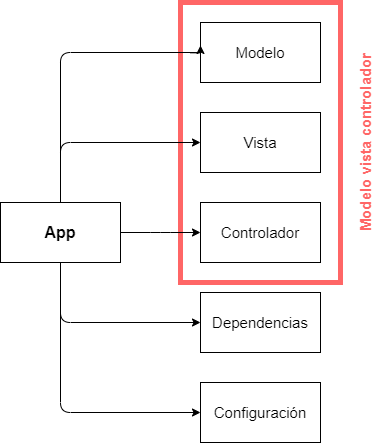
\includegraphics[width=0.6\textwidth]{imagenes/Estructura_carpetas.png}
\caption{Estructura de carpetas de la aplicación}
\label{fig:estructuraCarpetas}
\end{figure}

\subsection{Diagrama de clases}
Para facilitar la comprensión y que los diagramas se puedan interpretar de manera más sencilla, el diagrama de clases se va a dividir en cuatro partes. 
\begin{enumerate}
    \item Análisis: Esta parte se corresponde con el análisis de los mensajes. Estaría dentro del controlador del index y es la parte encargada de extraer los patrones.
    \item Controladores.
    \item Modelos.
    \item Vistas.
\end{enumerate}
\subsubsection{Análisis}
La parte del análisis está compuesta por tres partes (Ver figura \ref{fig:DC_anslisis}):
\begin{enumerate}
    \item Analyzer: Esta clase es la encargada de leer el mensaje en función del formato. 
    \item PatternSearcher: Es la clase encargada de buscar y extraer los patrones mediante las expresiones regulares que están almacenadas en la constante \textit{PATTERNS}. También valida que en el caso de los dominios (O los enlaces o las direcciones de correo) tentan un TDL correcto. 
    \item PatternContainer: En esta clase se almacenarán todos los patrones encargados. Evitará que haya repetidos, añadirá las características y las relaciones necesarias y se encargará de almacenar los datos en la base de datos mendiante el método \textit{save()} 
\end{enumerate}

\begin{figure}[htb]
    \centering
    %\includegraphics[width=0.5\textwidth]{spiral}
    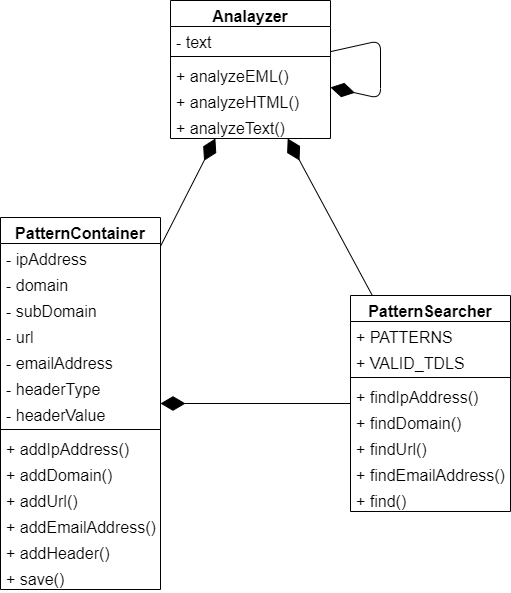
\includegraphics[width=0.6\textwidth]{imagenes/DiagramasClases/Analizador.png}
\caption{Estructura de carpetas de la aplicación}
\label{fig:DC_anslisis}
\end{figure}

\subsubsection{Controladores}
Los controladores permiten al usuario navegar por la web, en el controlador index es donde se permite al usuario enviar a analizar los correos, los demás son de consulta (correos, direcciones IP, dominios, enlaces y direcciones de correo).

Un ejemplo de controlador sería el código \ref{Codigo:controlador}

\begin{lstlisting}[
    language=PHP,
    breaklines, 
    caption={Ejemplo de controlador}, 
    label={Codigo:controlador}, 
    captionpos=b]
    class Domain extends Controller
    {	
        function __construct($request){
            parent::__construct('Domain.html', $request);
        }
        public function render(){

            $value = $this->request->getNextElement();
            if($value){
                $info = DataAccessObjectFactory::getDataAccessObject("DomainDAO_SQL_PDO")->getInfo($value);
                $this->addArgument("info", $info);
            }
            return parent::renderDirectly();
        }
    }
\end{lstlisting}

Todos los controladores heredan de una clase abstracta llamada Controller (Ver figura \ref{fig:DC_controladores}), en ella se almacenan todos los métodos genéricos, como la llamada a la librería de Twig o el nombre de la vista. También se crea un objeto Request en el que almacena información sobre la dirección en la que el usuario a clicado, esto permite al controlador saber qué vista debe generar y a qué modelo llamar. 

\paragraph{Clase Controller}
De esta clase destacan los siguientes métodos: 
\begin{itemize}
    \item notFound: se utiiza si se intenta acceder a una URL que el controlados no conoce. 
    \item addArgument: permite a las clases que heredan de ella añadir argumentos que se pasarán a la vista.
    \item render: es el método que genera la vista y la envía una vez que tiene todos los argumentos necesarios para generarla. 
\end{itemize}

\paragraph{Clase Request}
De esta clase destacan los siguientes métodos: 
\begin{itemize}
    \item getMethod: indica si el método con el que se hace la petición a Apache es get o Post.
    \item getNextElement: devuelve la siguiente parte del path si este está separado mediante ``\verb!/!''.
\end{itemize}

\begin{figure}[htb]
    \centering
    %\includegraphics[width=0.5\textwidth]{spiral}
    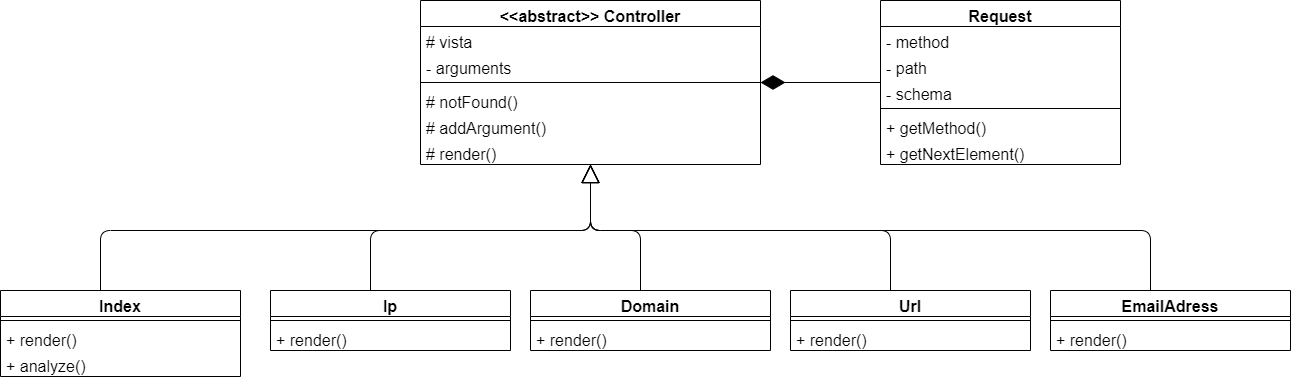
\includegraphics[width=0.8\textwidth]{imagenes/DiagramasClases/Controladores.png}
\caption{Diagrama de clases de los controladores}
\label{fig:DC_controladores}
\end{figure}

\subsubsection{Modelos}
Los modelos son los únicos encargados de interactuar con la base de datos, para hacer esto se ha hecho uso de la clase PDO de PHP, ya que aporta seguridad respecto a mysqli \cite{why_pdo_vs_msqli} y permite una migración sencilla a otro tipo de gestor de base de datos, como ya se ha mencionado (Ver apartado \ref{php_bases_de_datos}).

Para esto se ha utilizado la figura del Objeto de acceso a datos (DAO del inglés Data Access Object). Para evitar duplicar código, se ha creado una clase abstracta genérica llamada DataAccessObjectPDO de la cual extenderán las demás (Ver figura \ref{fig:DC_modelos}).

Esta clase está compuesta por un objeto de la clase DataBasePDO, en él se leerá un archivo de configuración con los parámetros de conexión a la base de datos. 
El separar estos dos objetos se hace para que puedan coexistir dos bases de datos al mismo tiempo.

\paragraph{Clase DataAccessObjectPDO}

De esta clase destacan los siguientes métodos: 
\begin{itemize}
    \item getConnection: Se utiliza para realizar la conexión con la base de datos. 
    \item getConnectionReadOnly: Es similar al método anterior, pero no se podrán leer datos.
    \item getItems: Es un método genérico para poder obtener todos los datos de la tabla del modelo actual.
    \item pagination: permite obtener una fracción de los datos de la tabla del modelo actual.
    \item prepare: genera una consulta preparada. 
    \item hash: se utiliza para generar el hash dado el valor. 
    \item findOrInsertFromArrayValues: permite obtener información a partir de un array de datos y en caso de no encontrarse, se insertan los elementos. 
    \item insertOrUpdateFromArrayValues: Se inserta un array de datos y en caso de existir ya el elemento, lo actualiza. 
\end{itemize}

Las clases que hereden de esta, tendrán que implementar dos métodos, \textit{getInfo()}, que se usa para obtener la información necesaria para la vista e \textit{insert()} que permite insertar objetos desde los métodos \textit{findOrInsertFromArrayValues()} o \textit{insertOrUpdateFromArrayValues()}. 


\begin{figure}[htb]
    \centering
    %\includegraphics[width=0.5\textwidth]{spiral}
    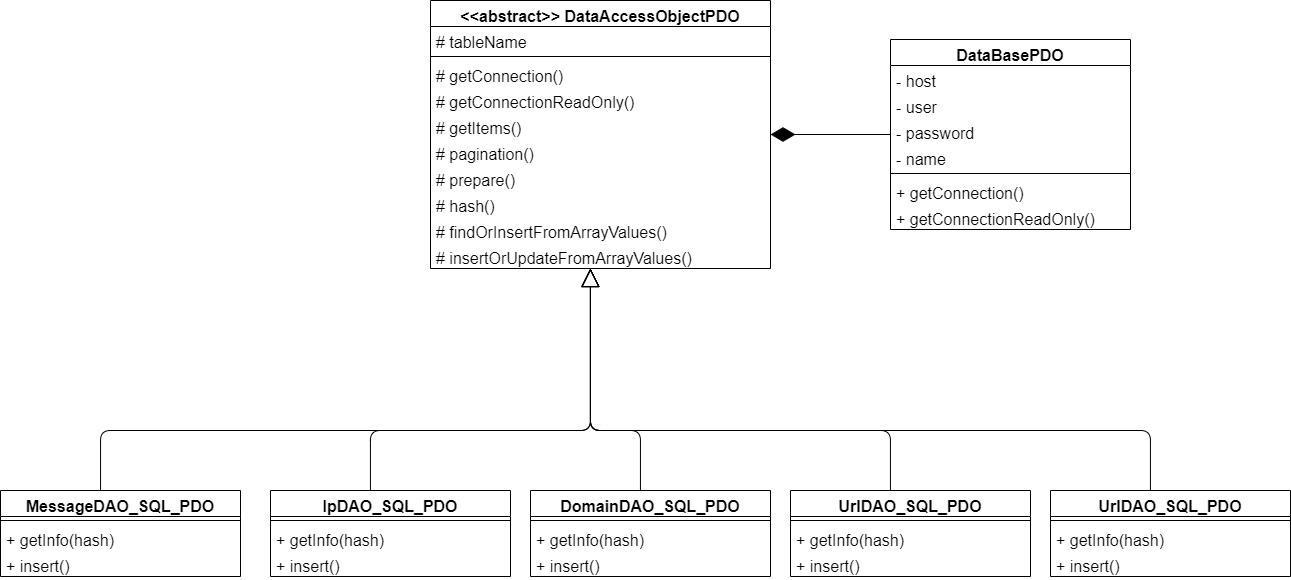
\includegraphics[width=0.8\textwidth]{imagenes/DiagramasClases/Modelos.png}
\caption{Diagrama de clases de los modelos}
\label{fig:DC_modelos}
\end{figure}

\subsubsection{Vistas}
Al ser una aplicación web, las vistas están hechas con HTML, CSS y JavaScript. En esta parte se ha utilizado Twig como gestor de plantillas y Bootstrap como librería para el diseño de la web. 

\paragraph{Twig}
Twig es un gestor de plantillas desarrollado por Symfony \cite{Twig} para PHP. Esto facilita la reutilización de código y el paso de información del modelo a la vista.

Gracias a la propiedad de herencia de Twig \cite{twig_extends}, se ha creado una plantilla base de la que heredarán las demás, de esta manera toda la información que es común se mantiene a lo largo de todas las vistas sin tener que repetir código, como por ejemplo la parte del header o del footer (ver figura \ref{fig:DC_vistas}). También se importará Bootstrap. 

\paragraph{Bootstrap}
Bootstrap es una librería desarrollada por Twitter con una gran cantidad de opciones y facilidades para el diseño web \cite{Bootstrap}. 
Se ha utilizado sobre todo para hacer la web adaptable a dispositivos móviles.

\begin{figure}[htb]
    \centering
    %\includegraphics[width=0.5\textwidth]{spiral}
    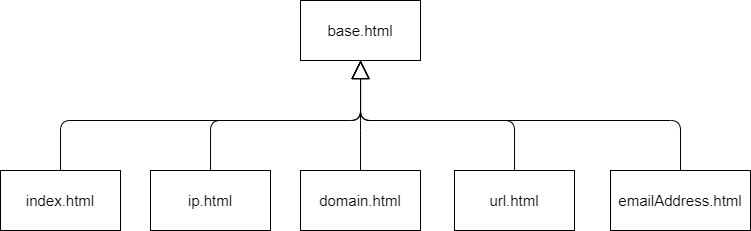
\includegraphics[width=0.8\textwidth]{imagenes/DiagramasClases/Vistas.png}
\caption{Diagrama de clases de las vistas}
\label{fig:DC_vistas}
\end{figure}

\subsection{Diagrama de flujo}
\subsubsection{Modelo Modelo-Vista-Controlador}\label{diagrama_MVC}
El modelo Modelo-Vista-Controlador se puede explicar mediante la secuencia sigueinte (Ver figura \ref{fig:MVC}): 
\begin{enumerate}
    \item El cliente realiza una acción que es capturada por el controlador. 
    \item El controlador elige un modelo, que se encarga de acceder a la base de datos y obtener la información necesaria. 
    \item El modelo le envía la información obtenida al controlador. 
    \item El controlador elige la vista adecuada y le pasa la información recibida del modelo. 
    \item La vista interpreta la información, en base a ella genera la vista final y se la envía al controlador. 
    \item El controlador le envía la vista ya formada al cliente. 
\end{enumerate}

\begin{figure}[htb]
    \centering
    %\includegraphics[width=0.5\textwidth]{spiral}
    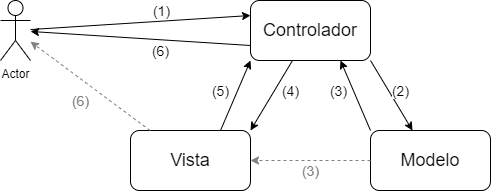
\includegraphics[width=0.8\textwidth]{imagenes/DiagramasFlujo/Modelo_Vista_Controlador.png}
\caption{Diagrama de flujo del modelo Modelo-Vista-Controlador}
\label{fig:MVC}
\end{figure}

\subsubsection{Diagrama de flujo al llegar un nuevo mensaje}
Al llegar un nuevo mensaje se siguen los siguientes pasos: 
\begin{enumerate}
    \item Se consulta si el correo ya ha sido analizado, en caso de haber sido analizado, se devuelve la información que haya en la base de datos.
    \item En caso de no haber sido analizado, en función del formato del mensaje se siguen los siguientes pasos.
        \begin{enumerate}
            \item EML: Si el formato es EML y tiene algún mensaje en el interior, se enviarán al punto 1 todos los mensajes que tengan.
            A continuación se analizarán las cabeceras, extrayendo por un lado el tipo y por otro el valor. 
            \begin{verbatim}
<Tipo de cabecera>:<valor>
            \end{verbatim}
            Dentro de valor se intentarán extraer todos los posibles patrones como si se tratase de un texto. 
            \item HTML: Si el mensaje está en formato HTML se observarán las etiquetas <a>, en concreto el valor del atributo “href” y del texto mostrado al usuario. 
            \item Texto plano: Si el formato es texto plano, simplemente se extraen todos los patrones mediante expresiones regulares y se almacenan.
        \end{enumerate}
\end{enumerate}

Hay que tener en cuenta que un texto en formato EML puede tener contenidos varios textos en varios formatos. Ver figura \ref{fig:nuevoMensaje}

\begin{figure}[htb]
    \centering
    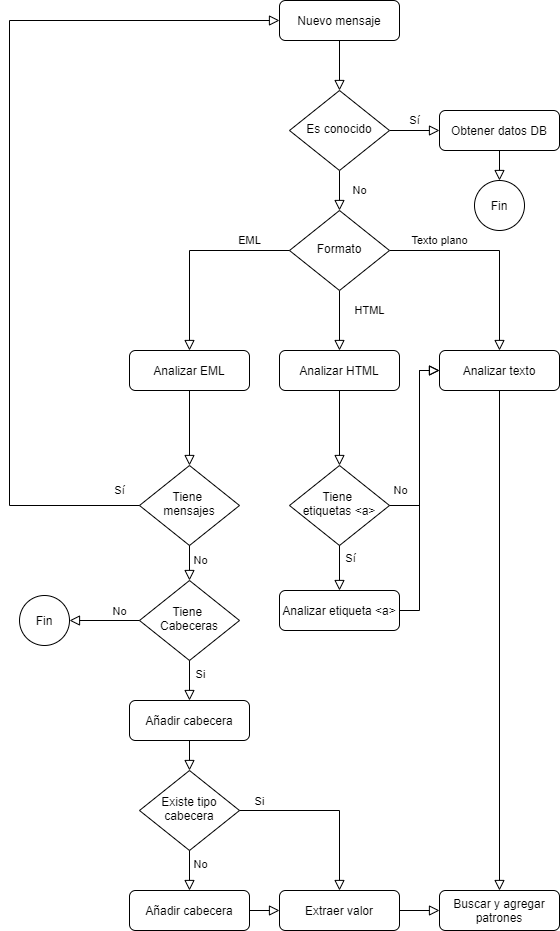
\includegraphics[width=0.8\textwidth]{imagenes/DiagramasFlujo/NuevoMensaje.png}
\caption{Diagrama de flujo cuando llega un nuevo mensaje}
\label{fig:nuevoMensaje}
\end{figure}

\cprotect\subsubsection{Diagrama de flujo para analizar una etiqueta \verb!<a>!}

Para analizar la etiqueta \verb!<a>!, esta debe tener un atributo “href” y texto. Si ambos coinciden, no se hace nada, en caso contrario, se aumenta el score del patrón del atributo “href”. Ver figura \ref{fig:etiquetas_a}.

\begin{figure}[htb]
    \centering
    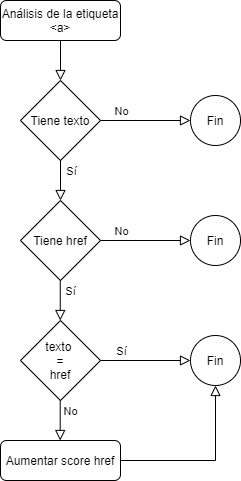
\includegraphics[width=0.4\textwidth]{imagenes/DiagramasFlujo/etiqueta_a.png}
\caption{Diagrama de flujo para analizar las etiquetas 
\texttt{<a>}}
\label{fig:etiquetas_a}
\end{figure}


\subsubsection{Diagrama de flujo para analizar una etiqueta}
En este apartado se irá comprobado si en el texto se encuentran patrones de los que se han obtenido las expresiones regulares en el punto \ref{imp:expresiones_regulares}. En caso de que haya, se comprobará si tiene características maliciosas como las mencionadas en el punto \ref{patrones_maliciosos}, en caso de tener alguna de ellas, se aumentará su score y se almacenará.  Ver figura \ref{fig:patrones}.

\begin{figure}[htb]
    \centering
    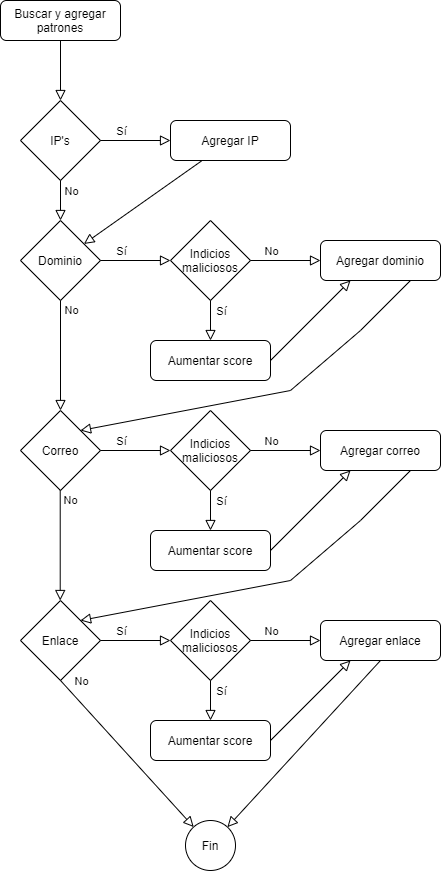
\includegraphics[width=0.6\textwidth]{imagenes/DiagramasFlujo/Buscar_agregar_patrones.png}
\caption{Diagrama de flujo para buscar y almacenar patrones}
\label{fig:patrones}
\end{figure}
\clearpage
\section{Capturas de pantallas} \label{capturas}
\subsection{Index}
En la imagen \ref{fig:index} se puede ver la página inicial de la aplicación. 
En ella los usuarios pueden copiar y pegar el correo para que sea analizado, además deben indicar al sistema qué tipo de mensaje es (EML, HTML o texto).
\begin{figure}[htb]
    \centering
    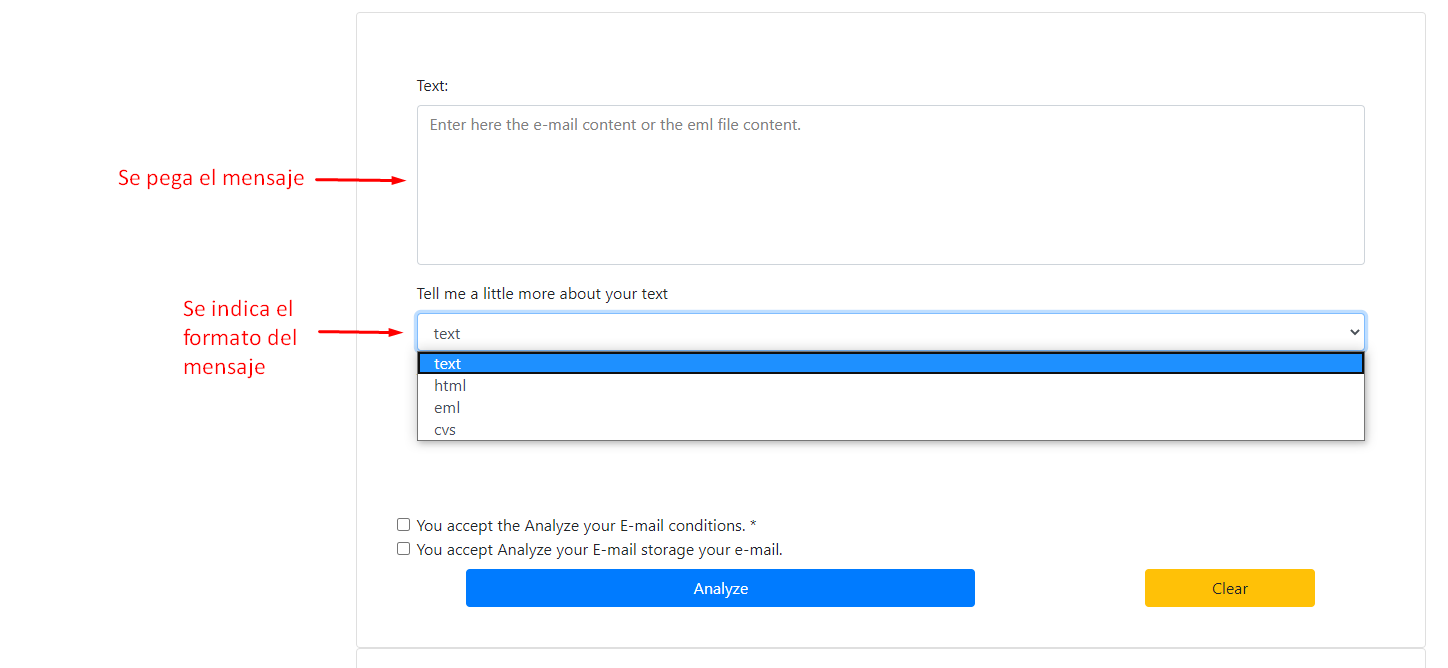
\includegraphics[width=\textwidth]{imagenes/capturasAplicacion/Analizar_mensaje.png}
\caption{Index de la aplicación}
\label{fig:index}
\end{figure}

\subsection{Mensaje}
Cuando un mensaje es analizado, el usuario verá algo parecido a las figuras \ref{fig:mensaje_datos} y \ref{fig:mensaje_patrones}. En la primera se puede ver la información básica del mensaje, como el formato, cuándo se añadió o cuándo se analizó. 

En la segunda figura \ref{fig:mensaje_patrones} se pueden ver qué patrones se han encontrado en dicho mensaje. Además, en caso de que el usuario quiera obtener más información sobre algún patrón en contro, simplemente podría clicar encima para ser redirigido a la página del patrón. 

\begin{figure}[htb]
    \centering
    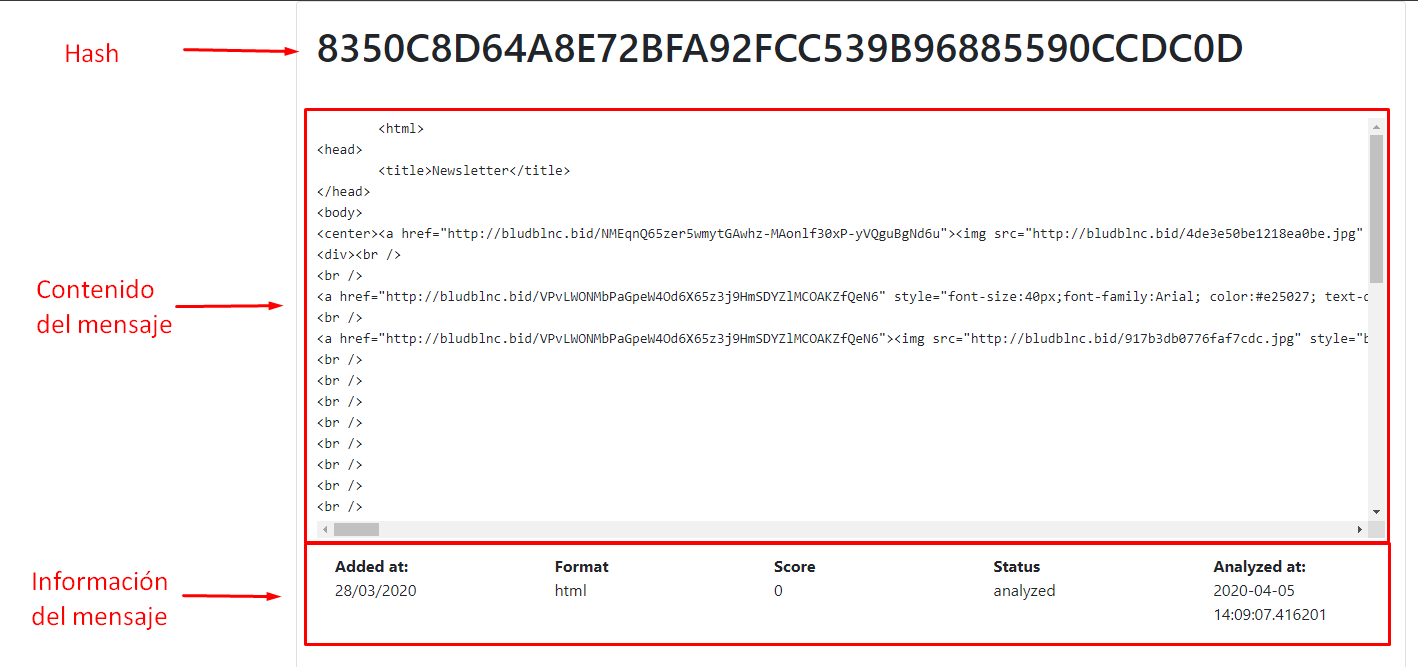
\includegraphics[width=0.9\textwidth]{imagenes/capturasAplicacion/Mensaje_info.png}
\caption{Vista de un mensaje: Información básica}
\label{fig:mensaje_datos}
\end{figure}

\begin{figure}[htb]
    \centering
    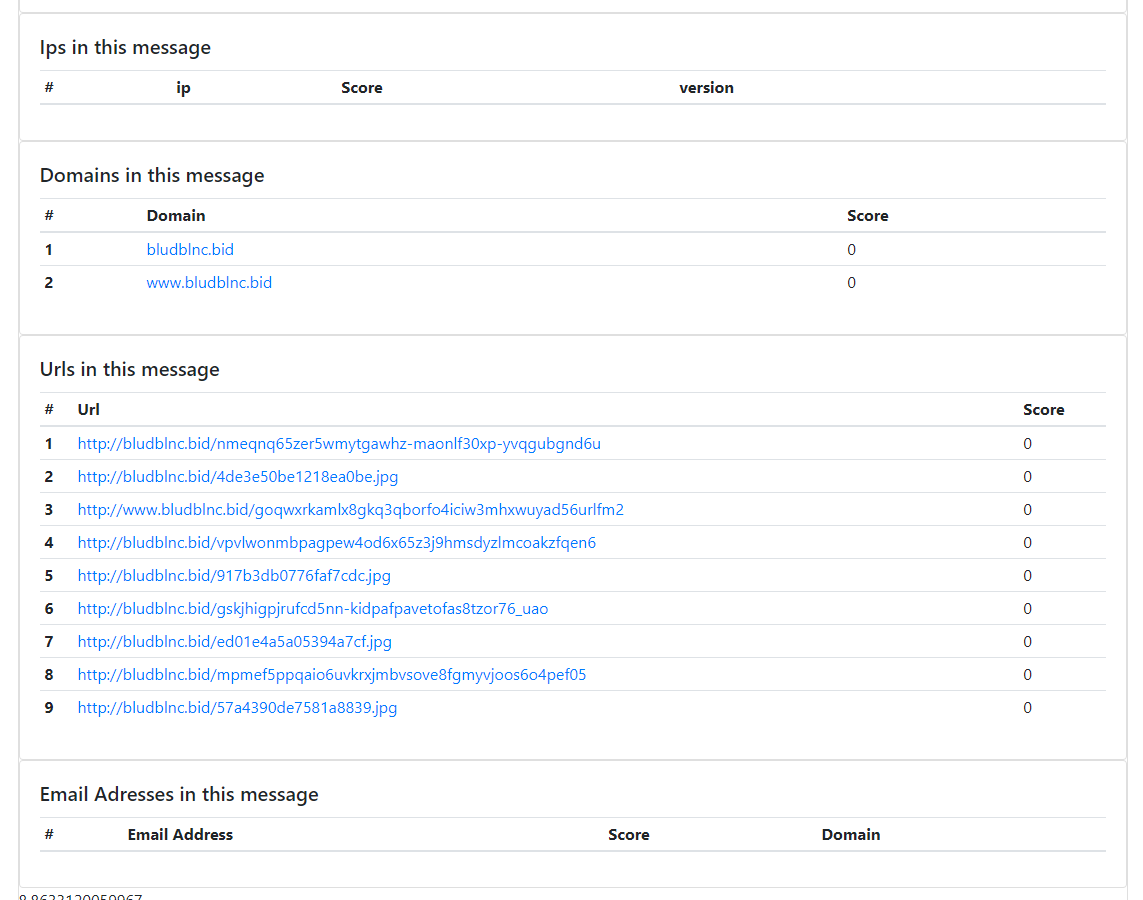
\includegraphics[width=0.9\textwidth]{imagenes/capturasAplicacion/Mensaje_patrones.png}
\caption{Vista de un mensaje: Patrones}
\label{fig:mensaje_patrones}
\end{figure}
\clearpage
\subsection{Dominio}
En el caso de los dominios, la información varía un poco dependiendo de si es un dominio (figura \ref{fig:dominio}) o un sundominio (figura \ref{fig:Subdominio}).

En caso de ser un subdominio, en la información básica aparecerá el dominio al que pertenece pudiendo navegar hacia él si se clica. 

Por otro lado, en caso de ser un dominio, aparecerán sus subdominios.

El resto de información como mensajes, enlaces, o direcciones de correo donde aparece este patrón, es idéntica y se puede navegar hacia ellos si se clica encima. 

\begin{figure}[htb]
    \centering
    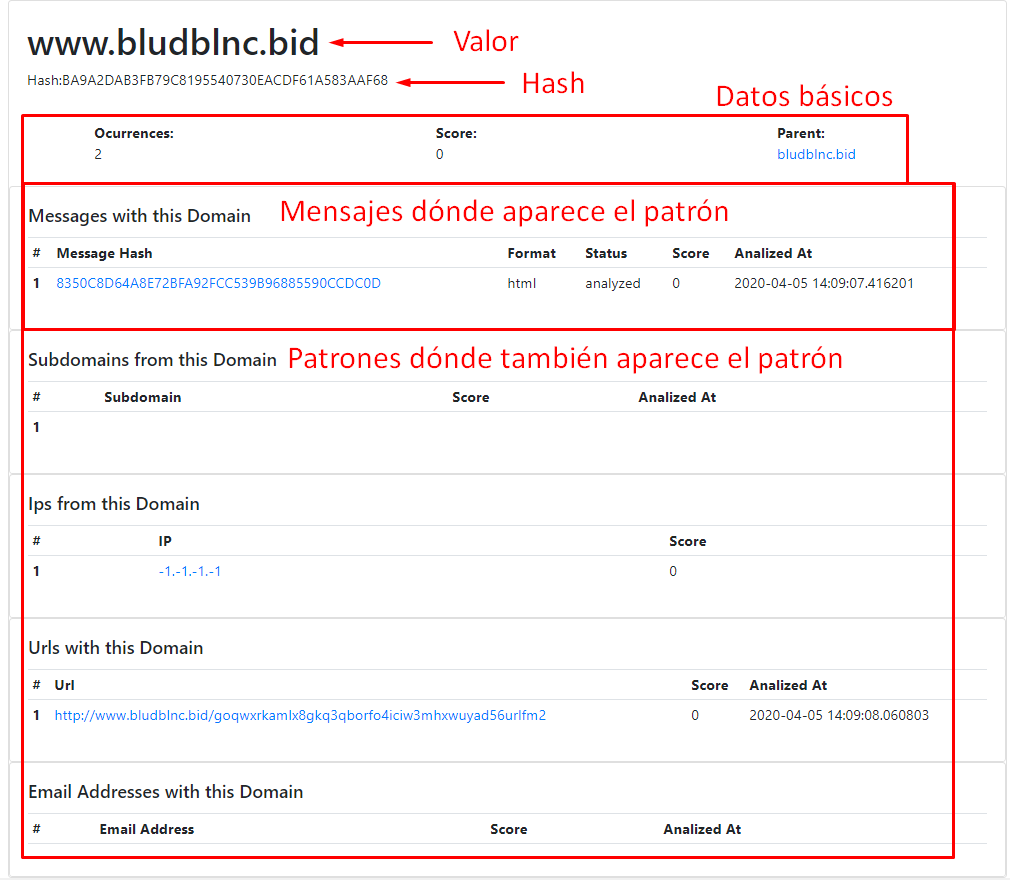
\includegraphics[width=0.9\textwidth]{imagenes/capturasAplicacion/Subdominio.png}
\caption{Vista de un subdominio.}
\label{fig:Subdominio}
\end{figure}


\begin{figure}[htb]
    \centering
    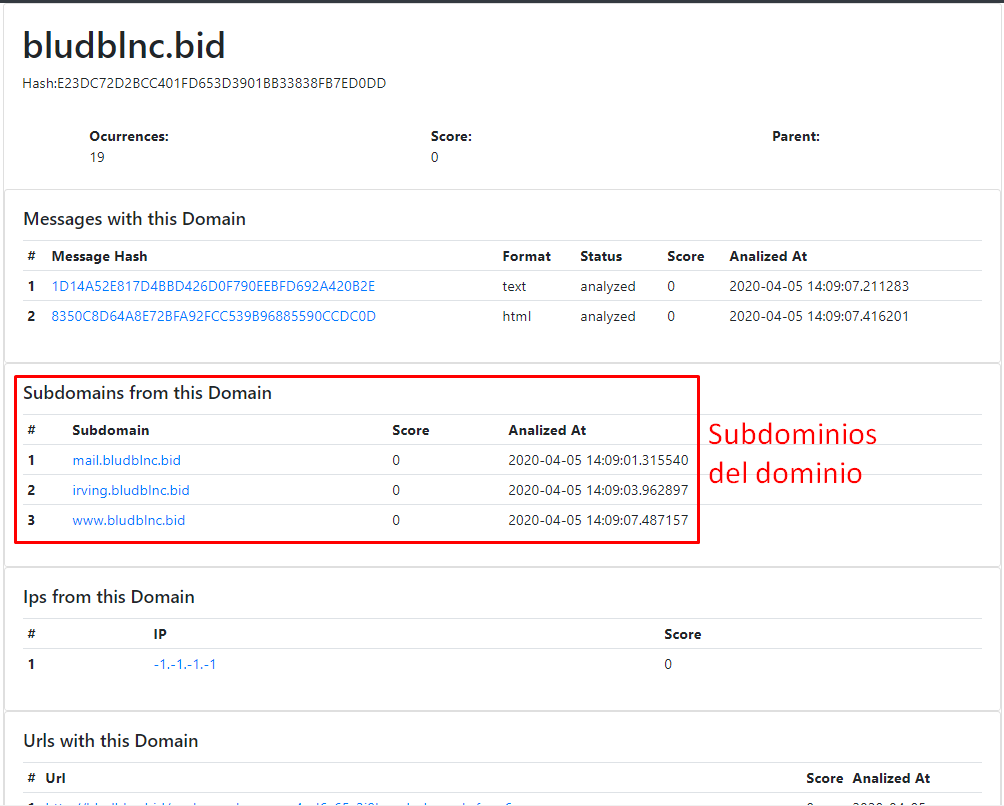
\includegraphics[width=0.9\textwidth]{imagenes/capturasAplicacion/Dominio.png}
\caption{Vista de un dominio.}
\label{fig:dominio}
\end{figure}

\clearpage
\subsection{Enlaces} \label{vista_enlaces}
En el caso de los enlaces, se ha integrado la plataforma con Virus Total, de modo que se puede analizar el enlace directamente desde la aplicación clicándo únicamente en el botón de \textit{Analyze} (Ver figuras \ref{fig:enlace} y \ref{fig:enlace_vt}).

\begin{figure}[htb]
    \centering
    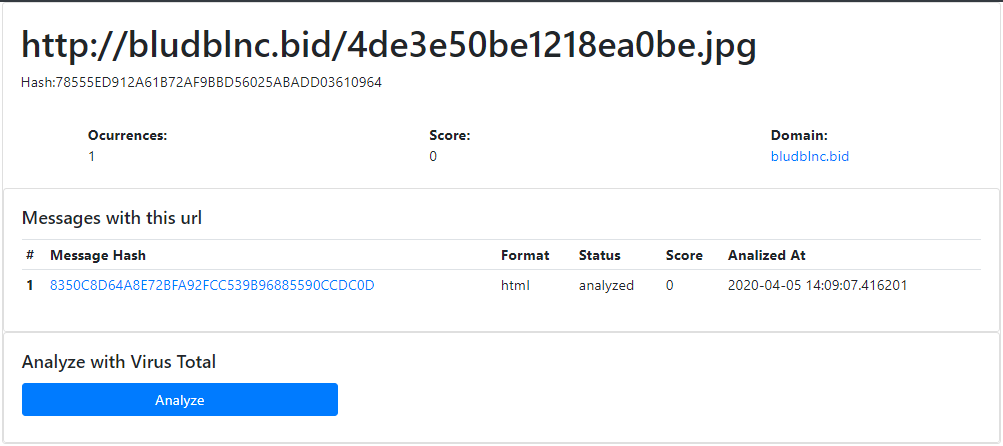
\includegraphics[width=0.8\textwidth]{imagenes/capturasAplicacion/Enlaces.png}
\caption{Vista de un enlace.}
\label{fig:enlace}
\end{figure}


\begin{figure}[htb]
    \centering
    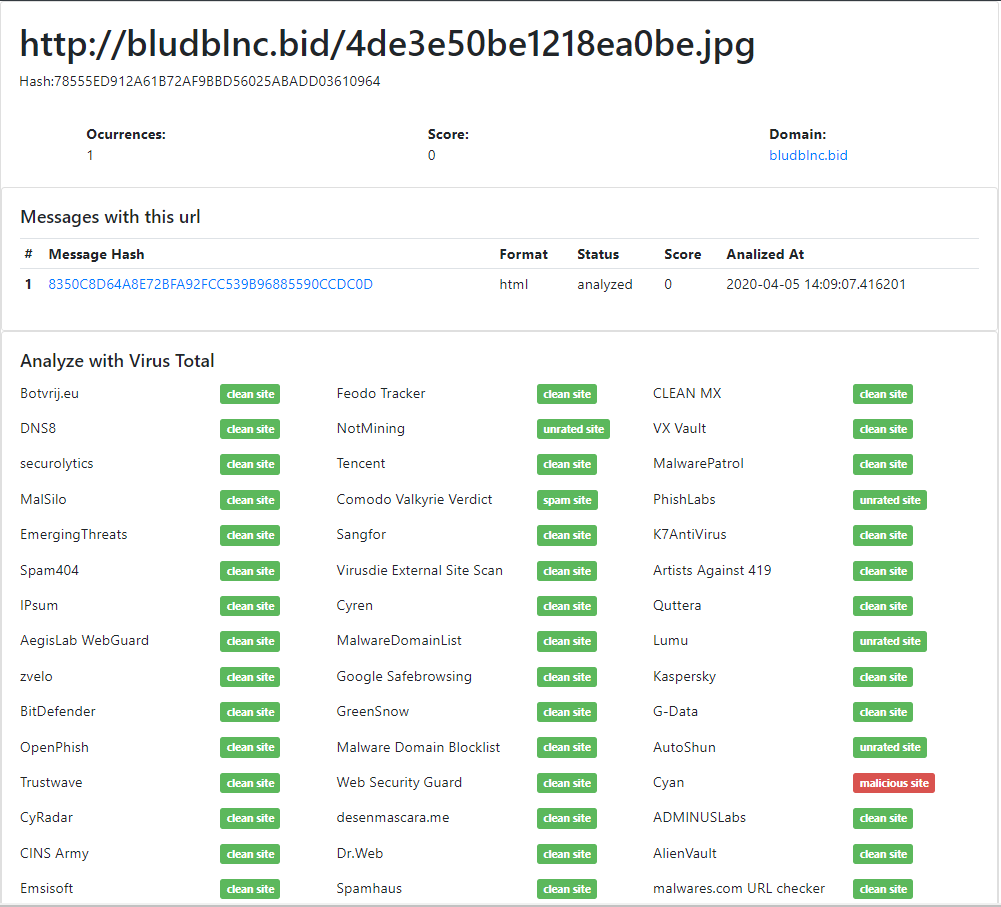
\includegraphics[width=0.8\textwidth]{imagenes/capturasAplicacion/Enlaces_virusTotal.png}
\caption{Vista de un enlace tras analizarlo con VirusTotal.}
\label{fig:enlace_vt}
\end{figure}

\clearpage
\subsection{Direcciones IP} \label{vista_ip}
Finalmente con las direcciones IP también se ha integrado el servicio de VirusTotal pudiendo analizar la dirección IP con este servicio (ver figuras \ref{fig:ip} y \ref{fig:ip_vt}).

\begin{figure}[htb]
    \centering
    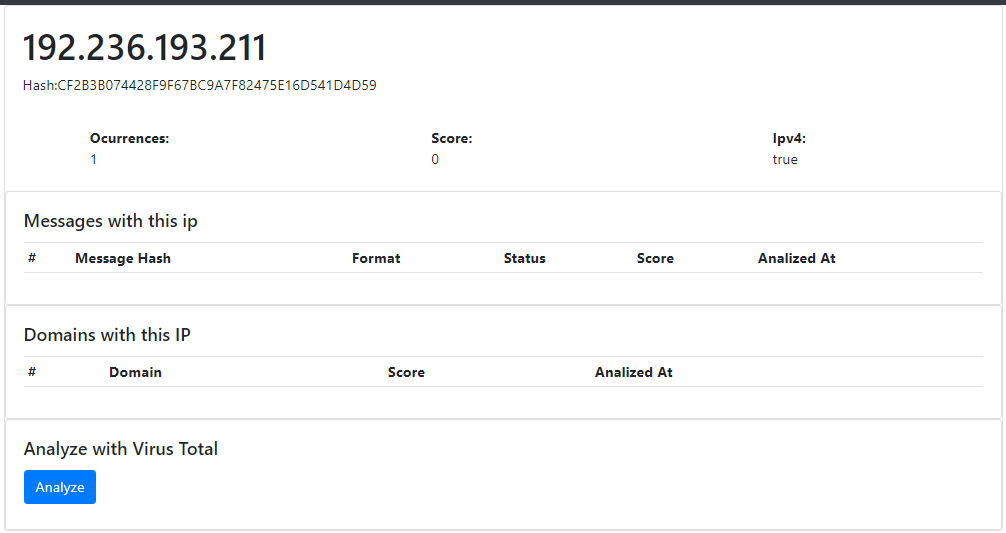
\includegraphics[width=0.8\textwidth]{imagenes/capturasAplicacion/IP.png}
\caption{Vista de una dirección IP.}
\label{fig:ip}
\end{figure}


\begin{figure}[htb]
    \centering
    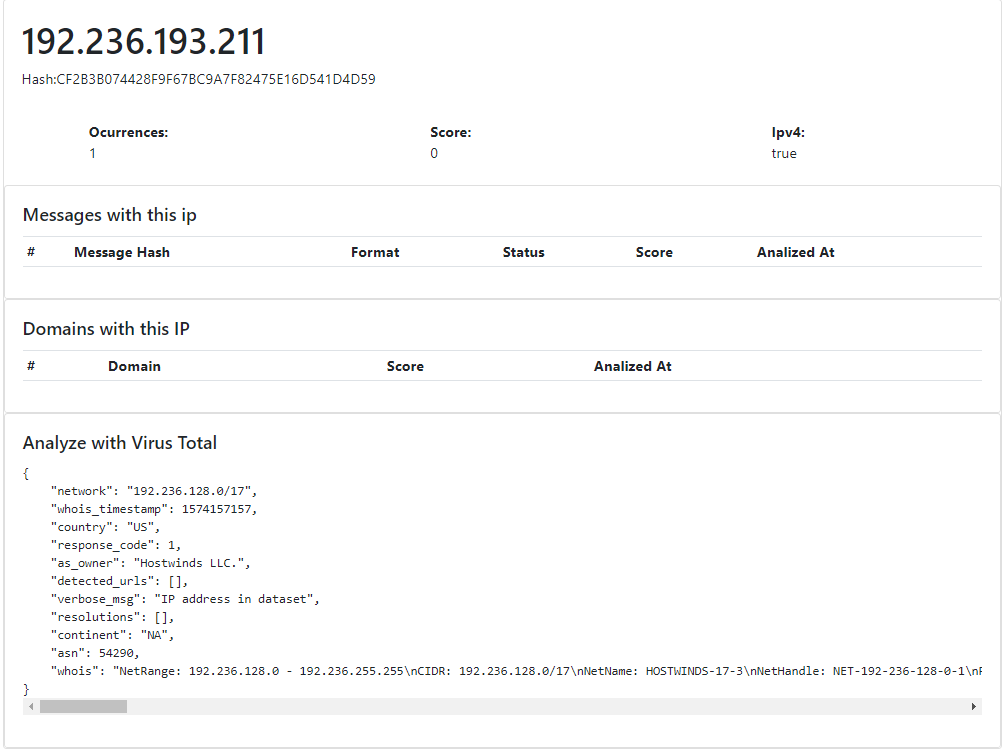
\includegraphics[width=0.8\textwidth]{imagenes/capturasAplicacion/IP_vt.png}
\caption{Vista de una dirección IP tras analizarla con VirusTotal.}
\label{fig:ip_vt}
\end{figure}
\appendix
\chapter{Documentos}
\section{Ejemplo formato EML}
\begin{lstlisting}[
    breaklines, 
    caption={Ejemplo archivo EML}, 
    label={Documento:eml_example}, 
    captionpos=b
    ]
Return-Path: <SRS0=v5D8h6=TB=rankgator.live=kelly@untroubled.org>
Delivered-To: bruce@home.untroubled.org
Received: from rankgator.live (rdns.bitacel.com [194.34.104.232])
  by pt02.futurequest.net ([69.5.6.173])
  with ESMTP via TCP; 01 May 2019 14:41:04 -0000
Message-ID: <xat683W4TM32ruh.ilcIL221JGS1tho@rankgator.live> 
From: "Arctic Pain Relief" <kelly@rankgator.live> 
Date: Wed, 01 May 2019 10:09:17 -0400 
MIME-Version: 1.0 
Subject: Are  you -part -of-- the-- world’s- biggest arthritis cover-up? 
To: "bruce@untroubled.org" <bruce@untroubled.org> 
Content-type: multipart/alternative; boundary="---=_Part_1426_87C624P49.F740FP9";
Content-Length: 1606

-----=_Part_1426_87C624P49.F740FP9
Content-Type: text/plain; format=flowed; charset="UTF-8"
Content-Transfer-Encoding: 7bit

Are you part of the world’s biggest arthritis cover-up?

http://efs5I69IX4S3elw.rankgator.live/208fdcae990695eb0665b0903677f315_8da8c95c-0101030c0001/1/

Are you part of the world’s biggest arthritis cover-up?

-----=_Part_1426_87C624P49.F740FP9
Content-Type: text/html; charset=us-ascii
Content-Transfer-Encoding: 7bit

<!DOCTYPE html PUBLIC "-//W3C//DTD HTML 4.01 Transitional//EN">
<html>
  <head>
    <title></title>
  </head>
  <body>
    <table>
      <tr>
        <td colspan='2' align='center' valign='middle' class='preview-mid'>
          <br>
          <center>
            <a href="http://sdvPL9B7FL5Hwfm.rankgator.live/208fdcae990695eb0665b0903677f315_8da8c95c-0101030c0001/1/"><img src="http://ifq7BTAN28Q1vfo.rankgator.live/images//4b128133049378e37097925975e252e1" border="0" alt=""></a>
          </center>
          <div align="center">
###STUFF##
            <font face="Verdana, Arial, Helvetica, sans-serif" size="1"><br>
            If you'd prefer not to receive future emails, <a href="http://pkvG0P5I93MHwgd.rankgator.live/208abda8ac8695eb0665b0903678f315_8da8c95c-0101030c0001/1/"><font color="#666666">Unsubscribe Here</font></a>.<br>
            616 Corporate Way, | Suite 2-5335 Valley Cottage | NY NY 10989</font>
          </div>
        </td>
      </tr>
    </table>
  </body>
</html>

<center>



<img src="http://pmsG8XP16WP5bqb.rankgator.live/2082301ea94695eb0665b090365f030b_8da8c95c-0101030c0001/2/">

-----=_Part_1426_87C624P49.F740FP9--
\end{lstlisting}
\chapter{Base de datos}
\section{Diagrama entidad relación}


\begin{figure}[H]
    \centering
    %\includegraphics[width=0.5\textwidth]{spiral}
    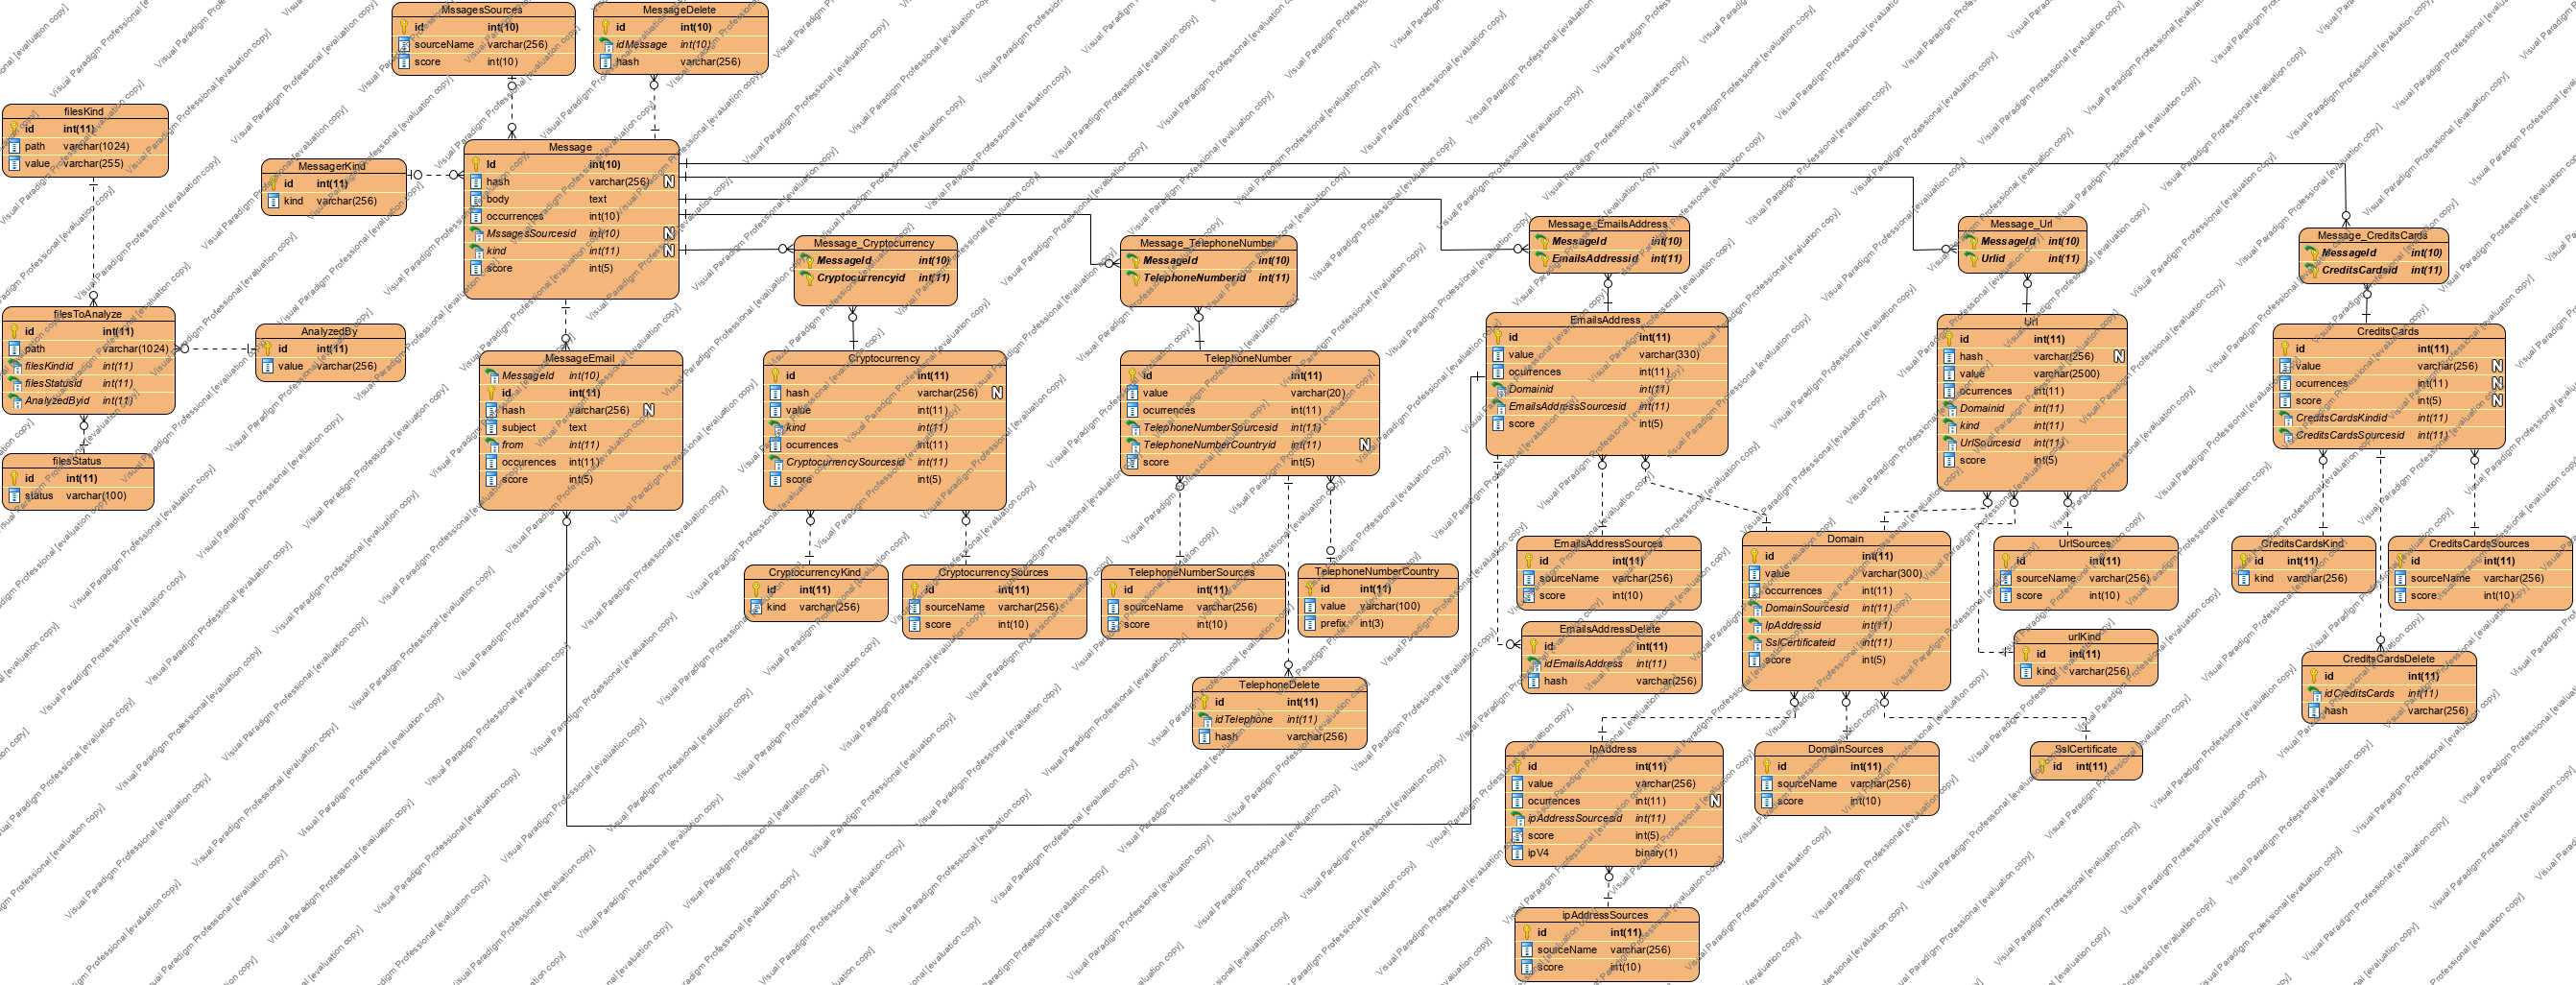
\includegraphics[scale=0.2, angle=90]{imagenes/Diagrama_entidad_relacion.png}
\caption{Diagrama entidad entidad relación de la Base de datos}
\end{figure}



\section{Tablas e índices}
\renewcommand{\lstlistingname}{Tabla}% Listing -> Algorithm

\subsection{Mensajes}
\subsubsection{Formato de los mensajes}
\begin{lstlisting}[
    language=SQL,
    breaklines, 
    caption={Tabla MessageFormat}, 
    label={Tabla:MessageFormat}, 
    captionpos=b
    ]
    create  table MessageFormat (
    id   tinyint UNSIGNED  not null auto_increment, 
    value varchar(256) not null, 
    primary key (id));
    INSERT INTO MessageFormat(value) VALUES ("eml");
    INSERT INTO MessageFormat(value) VALUES ("html");
    INSERT INTO MessageFormat(value) VALUES ("text");
    INSERT INTO MessageFormat(value) VALUES ("csv");
\end{lstlisting}

\subsubsection{Analizado por}
\begin{lstlisting}[
    language=SQL,
    breaklines, 
    caption={Tabla AnalyzedBy}, 
    label={Tabla:AnalyzedBy}, 
    captionpos=b
    ]
    create  table AnalyzedBy (
    id    tinyint UNSIGNED  not null auto_increment, 
    value varchar(256) not null, 
    primary key (id));
    INSERT INTO AnalyzedBy(value) VALUES ("php");
    INSERT INTO AnalyzedBy(value) VALUES ("node");
\end{lstlisting}

\subsubsection{Estado del mensaje}
\begin{lstlisting}[
    language=SQL,
    breaklines, 
    caption={Tabla MessageStatus}, 
    label={Tabla:MessageStatus}, 
    captionpos=b
    ]
    create  table MessageStatus (
    id     tinyint UNSIGNED  not null auto_increment, 
    value varchar(100) not null, 
    primary key (id));
    INSERT INTO MessageStatus(value) VALUES ("pending");
    INSERT INTO MessageStatus(value) VALUES ("analyzing");
    INSERT INTO MessageStatus(value) VALUES ("analyzed");
    INSERT INTO MessageStatus(value) VALUES ("error");
\end{lstlisting}

\subsubsection{Datos del mensaje}
\begin{lstlisting}[
    language=SQL,
    breaklines, 
    caption={Tabla MessageData}, 
    label={Tabla:MessageData}, 
    captionpos=b
    ]
    create  table MessageData (
    id            int UNSIGNED  not null auto_increment, 
    hash          binary(20) not null, 
    score         smallint default 0 not null, 
    format        tinyint UNSIGNED  not null, 
    analyzedBy    tinyint UNSIGNED  null DEFAULT NULL, 
    status        tinyint UNSIGNED  not null DEFAULT 1, 
    analysisTime  DECIMAL(9,6) null DEFAULT NULL,
    addeddAt      TIMESTAMP(6) NOT NULL DEFAULT CURRENT_TIMESTAMP(6),
    analyzedAt    TIMESTAMP(6) NULL DEFAULT NULL,
    updatedAt     TIMESTAMP(6) NULL DEFAULT NULL ON UPDATE CURRENT_TIMESTAMP(6),
    UNIQUE INDEX iq_messageData_hash (hash ASC),
    CONSTRAINT FK_MessageFormat_Message FOREIGN KEY (format) REFERENCES MessageFormat (id) ON DELETE NO ACTION ON UPDATE NO ACTION,
    CONSTRAINT FK_AnalyzedBy_Message FOREIGN KEY (analyzedBy) REFERENCES AnalyzedBy (id) ON DELETE NO ACTION ON UPDATE NO ACTION,
    CONSTRAINT FK_MessageStatus_Message FOREIGN KEY (status) REFERENCES MessageStatus (id) ON DELETE NO ACTION ON UPDATE NO ACTION,
    primary key (Id));
\end{lstlisting}

\subsubsection{Texto del mensaje}
\begin{lstlisting}[
    language=SQL,
    breaklines, 
    caption={Tabla MessageText}, 
    label={Tabla:MessageText}, 
    captionpos=b
    ]
    create  table MessageText (
    id            int UNSIGNED  not null auto_increment, 
    value         text CHARACTER SET utf8 COLLATE utf8_unicode_ci NOT null, 
    CONSTRAINT FK_MessageData_MessageText FOREIGN KEY (id) REFERENCES MessageData (id) ON DELETE CASCADE ON UPDATE NO ACTION,
    FULLTEXT ftidx_MessageText_value (value),
    primary key (id));
\end{lstlisting}

\subsubsection{Submensajes}
\begin{lstlisting}[
    language=SQL,
    breaklines, 
    caption={Tabla ChildMessages}, 
    label={Tabla:ChildMessages}, 
    captionpos=b
    ]
    create  table ChildMessages (
    parentId         int UNSIGNED  not null, 
    childId          int UNSIGNED  not null, 
    CONSTRAINT FK_MessageData_Message_ChildMessages_Parent FOREIGN KEY (parentId) REFERENCES MessageData (id) ON DELETE CASCADE ON UPDATE NO ACTION,
    CONSTRAINT FK_MessageData_Message_ChildMessages_Child FOREIGN KEY (childId) REFERENCES MessageData (id) ON DELETE CASCADE ON UPDATE NO ACTION,
    primary key (parentId, childId));
\end{lstlisting}

\subsection{Patrones}

\begin{lstlisting}[
    language=SQL,
    breaklines, 
    caption={Tablas de la información extraida y auxiliares}, 
    label={Tabla:elements}, 
    captionpos=b
    ]
    create  table IpAddress (
  id         int UNSIGNED  not null auto_increment, 
  hash       binary(20) not null, 
  value      varchar(50) not null, 
  score      smallint default 0 not null, 
  ipv4       tinyint(1) not null, 
  UNIQUE INDEX  iq_IpAddress_value (value ASC),
  UNIQUE INDEX  iq_IpAddress_hash (hash ASC),
  primary key (id));

create  table Domain (
  id          int UNSIGNED  not null auto_increment, 
  hash        binary(20) not null, 
  value       varchar(330) not null, 
  score       smallint default 0 not null, 
  analyzedAt  TIMESTAMP(6) NOT NULL DEFAULT CURRENT_TIMESTAMP(6),
  parentId    int UNSIGNED  null, 
  INDEX idx_domain_parentId (parentId ASC),
  UNIQUE INDEX iq_Domain_hash (hash ASC),
  primary key (id));
  ALTER TABLE Domain ADD CONSTRAINT fk_domain_parentId_id FOREIGN KEY (parentId) REFERENCES Domain (id) ON DELETE NO ACTION ON UPDATE NO ACTION;

create  table Domain_IpAddress (
  DomainId        int UNSIGNED  not null, 
  IpAddressId     int UNSIGNED  not null,
  CONSTRAINT FK_Domain__Domain_IpAddress FOREIGN KEY (DomainId) REFERENCES Domain (id) ON DELETE CASCADE ON UPDATE NO ACTION,
  CONSTRAINT FK_IpAddress__Domain_IpAddress FOREIGN KEY (IpAddressId) REFERENCES IpAddress (id) ON DELETE CASCADE ON UPDATE NO ACTION,
  primary key (DomainId, IpAddressId));


create  table EmailAddress (
  id          int UNSIGNED  not null auto_increment, 
  hash        binary(20) not null, 
  value       varchar(330) not null, 
  score       smallint default 0 not null, 
  analyzedAt  TIMESTAMP(6) NOT NULL DEFAULT CURRENT_TIMESTAMP(6),
  domain      int UNSIGNED  not null, 
  UNIQUE INDEX  iq_EmailAddress_hash (hash ASC),
  CONSTRAINT FK_Domain__EmailAddress FOREIGN KEY (domain) REFERENCES Domain (id) ON DELETE NO ACTION ON UPDATE NO ACTION,
  primary key (id));


create  table UrlType (
  id    tinyint UNSIGNED  not null auto_increment, 
  value varchar(256) not null, 
  primary key (id));

INSERT INTO UrlType(value) VALUES ("link");
INSERT INTO UrlType(value) VALUES ("img");
INSERT INTO UrlType(value) VALUES ("video");

create  table Url (
  id          int UNSIGNED  not null auto_increment, 
  hash        binary(20) not null, 
  value       varchar(2500) not null, 
  score       smallint default 0 not null, 
  analyzedAt  TIMESTAMP(6) NOT NULL DEFAULT CURRENT_TIMESTAMP(6),
  domain      int UNSIGNED  not null, 
  type        tinyint UNSIGNED  not null, 
  UNIQUE INDEX  iq_Url_hash (hash ASC),
  CONSTRAINT FK_Domain__Url FOREIGN KEY (domain) REFERENCES Domain (id) ON DELETE NO ACTION ON UPDATE NO ACTION,
  primary key (id));

create  table MessageHeaderTypes (
  id                      mediumint UNSIGNED  not null auto_increment, 
  value                   text not null, 
  primary key (id));

create  table MessageHeaderValues (
  id                      int UNSIGNED  not null auto_increment, 
  hash                    binary(20) not null, 
  value                   text not null, 
  emailHeaderTypesId      mediumint UNSIGNED  not null, 
  UNIQUE INDEX  iq_Url_hash (hash ASC),
  INDEX idx_MessageHeaderValues_emailHeaderTypesId (emailHeaderTypesId ASC),
  CONSTRAINT FK_MessageHeaderTypes__MessageHeaderValues FOREIGN KEY (emailHeaderTypesId) REFERENCES MessageHeaderTypes (id) ON DELETE NO ACTION ON UPDATE NO ACTION,
  primary key (id));




create  table MessageDelete (
  id        int UNSIGNED  not null auto_increment, 
  idMessage int UNSIGNED  not null, 
  hash      varchar(256) not null, 
  CONSTRAINT FK_MessageData_MessageDelete FOREIGN KEY (idMessage) REFERENCES MessageData (id) ON DELETE CASCADE ON UPDATE NO ACTION,
  primary key (id));

create  table MessageDataSources (
  id         SMALLINT UNSIGNED  not null auto_increment, 
  value varchar(100) not null, 
  score      smallint default 0 not null, 
  UNIQUE INDEX uq_MessageDataSources_value (value DESC),
  primary key (id));
INSERT INTO MessageDataSources(value) VALUES ("fromWeb");
INSERT INTO MessageDataSources(value) VALUES ("onEml");


create  table MessageData_MessageDataSources (
  MessageDataId         int UNSIGNED  not null, 
  MessageDataSourcesId  SMALLINT UNSIGNED  not null,
  date              TIMESTAMP(6) NOT NULL DEFAULT CURRENT_TIMESTAMP(6),
  CONSTRAINT FK_MessageData__Message_MessageDataSources FOREIGN KEY (MessageDataId) REFERENCES MessageData (id) ON DELETE CASCADE ON UPDATE NO ACTION,
  CONSTRAINT FK_MessageDataSources__Message_MessageDataSources FOREIGN KEY (MessageDataSourcesId) REFERENCES MessageDataSources (id) ON DELETE NO ACTION ON UPDATE NO ACTION,
  primary key (MessageDataId, MessageDataSourcesId, date));






create  table IpAddressSources (
  id         smallint UNSIGNED  not null auto_increment, 
  value varchar(100) not null, 
  score      smallint  default 0 not null, 
  UNIQUE INDEX uq_IpAddressSources_value (value DESC),
  primary key (id));
INSERT INTO IpAddressSources(value) VALUES ("textAnalysis");
INSERT INTO IpAddressSources(value) VALUES ("emlHeaders");
INSERT INTO IpAddressSources(value) VALUES ("onDomain");
INSERT INTO IpAddressSources(value) VALUES ("aHref");
INSERT INTO IpAddressSources(value) VALUES ("aText");


create  table IpAddress_IpAddressSources (
  IpAddressId         int UNSIGNED  not null, 
  IpAddressSourcesId smallint UNSIGNED  not null,
  date              TIMESTAMP(6) NOT NULL DEFAULT CURRENT_TIMESTAMP(6),
  CONSTRAINT FK_IpAddress__IpAddress_IpAddressSources FOREIGN KEY (IpAddressId) REFERENCES IpAddress (id) ON DELETE CASCADE ON UPDATE NO ACTION,
  CONSTRAINT FK_IpAddressSources__IpAddress_IpAddressSources FOREIGN KEY (IpAddressSourcesId) REFERENCES IpAddressSources (id) ON DELETE NO ACTION ON UPDATE NO ACTION,
  primary key (IpAddressId, IpAddressSourcesId, date));



create  table DomainSources (
  id         smallint UNSIGNED  not null auto_increment, 
  value varchar(100) not null, 
  score      smallint  default 0 not null, 
  UNIQUE INDEX uq_DomainSources_value (value DESC),
  primary key (id));
INSERT INTO DomainSources(value) VALUES ("textAnalysis");
INSERT INTO DomainSources(value) VALUES ("emlHeaders");
INSERT INTO DomainSources(value) VALUES ("onUrl");
INSERT INTO DomainSources(value) VALUES ("onSubdomain");
INSERT INTO DomainSources(value) VALUES ("onEmailAddress");
INSERT INTO DomainSources(value) VALUES ("aHref");
INSERT INTO DomainSources(value) VALUES ("aText");

create  table Domain_DomainSources (
  DomainId          int UNSIGNED  not null, 
  DomainSourcesId   smallint UNSIGNED  not null,
  date              TIMESTAMP(6) NOT NULL DEFAULT CURRENT_TIMESTAMP(6),
  CONSTRAINT FK_Domain__Domain_DomainSources FOREIGN KEY (DomainId) REFERENCES Domain (id) ON DELETE CASCADE ON UPDATE NO ACTION,
  CONSTRAINT FK_DomainSources__Domain_DomainSources FOREIGN KEY (DomainSourcesId) REFERENCES DomainSources (id) ON DELETE NO ACTION ON UPDATE NO ACTION,
  primary key (DomainId, DomainSourcesId, date));

create  table DomainMaliciousChecks (
  id         smallint UNSIGNED  not null auto_increment, 
  value      varchar(250) not null, 
  score      smallint default 0 not null, 
  primary key (id));

create  table Domain_DomainMaliciousChecks (
  DomainId                int UNSIGNED  not null, 
  DomainMaliciousChecksId smallint UNSIGNED  not null,
  CONSTRAINT FK_Domain__Domain_DomainMaliciousChecks FOREIGN KEY (DomainId) REFERENCES Domain (id) ON DELETE CASCADE ON UPDATE NO ACTION,
  CONSTRAINT FK_DomainMaliciousChecks__Domain_DomainMaliciousChecks FOREIGN KEY (DomainMaliciousChecksId) REFERENCES DomainMaliciousChecks (id) ON DELETE NO ACTION ON UPDATE NO ACTION,
  primary key (DomainId, DomainMaliciousChecksId));




create  table EmailAddressDelete (
  id        int UNSIGNED  not null auto_increment, 
  idEmailAddress int UNSIGNED  not null, 
  hash      varchar(256) not null, 
  CONSTRAINT FK_EmailAddress_EmailAddressDelete FOREIGN KEY (idEmailAddress) REFERENCES EmailAddress (id) ON DELETE CASCADE ON UPDATE NO ACTION,
  primary key (id));

create  table EmailAddressSources (
  id         smallint UNSIGNED  not null auto_increment, 
  value varchar(100) not null, 
  score      smallint default 0 not null, 
  UNIQUE INDEX uq_EmailAddressSources_value (value DESC),
  primary key (id));
INSERT INTO EmailAddressSources(value) VALUES ("textAnalysis");
INSERT INTO EmailAddressSources(value) VALUES ("emlHeaders");
INSERT INTO EmailAddressSources(value) VALUES ("aHref");
INSERT INTO EmailAddressSources(value) VALUES ("aText");

create  table EmailAddress_EmailAddressSources (
  EmailAddressId          int UNSIGNED  not null, 
  EmailAddressSourcesId   smallint UNSIGNED  not null,
  date                    TIMESTAMP(6) NOT NULL DEFAULT CURRENT_TIMESTAMP(6),
  CONSTRAINT FK_EmailAddress__EmailAddress_EmailAddressSources FOREIGN KEY (EmailAddressId) REFERENCES EmailAddress (id) ON DELETE CASCADE ON UPDATE NO ACTION,
  CONSTRAINT FK_EmailAddressSources__EmailAddress_EmailAddressSources FOREIGN KEY (EmailAddressSourcesId) REFERENCES EmailAddressSources (id) ON DELETE NO ACTION ON UPDATE NO ACTION,
  primary key (EmailAddressId, EmailAddressSourcesId, date));

create  table EmailAddressMaliciousChecks (
  id         smallint UNSIGNED  not null auto_increment, 
  value      varchar(250) not null, 
  score      smallint default 0 not null, 
  primary key (id));

create  table EmailAddress_EmailAddressMaliciousChecks (
  EmailAddressId                int UNSIGNED  not null, 
  EmailAddressMaliciousChecksId smallint UNSIGNED  not null,
  CONSTRAINT FK_EmailAddress__EmailAddress_EmailAddressMaliciousChecks FOREIGN KEY (EmailAddressId) REFERENCES EmailAddress (id) ON DELETE CASCADE ON UPDATE NO ACTION,
  CONSTRAINT FK_EmailAddressMC__EmailAddress_EmailAddressMC FOREIGN KEY (EmailAddressMaliciousChecksId) REFERENCES EmailAddressMaliciousChecks (id) ON DELETE NO ACTION ON UPDATE NO ACTION,
  primary key (EmailAddressId, EmailAddressMaliciousChecksId));
  
create  table EmailAddress_href_value (
  href         int UNSIGNED  not null, 
  text          int UNSIGNED  not null, 
  CONSTRAINT FK_EmailAddress__EmailAddress_href_value_href FOREIGN KEY (href) REFERENCES EmailAddress (id) ON DELETE CASCADE ON UPDATE NO ACTION,
  CONSTRAINT FK_EmailAddress__EmailAddress_href_value_text FOREIGN KEY (text) REFERENCES EmailAddress (id) ON DELETE CASCADE ON UPDATE NO ACTION,
  primary key (href, text));




create  table MessageData_IpAddress (
  MessageDataId   int UNSIGNED  not null, 
  IpAddressId     int UNSIGNED  not null,
  CONSTRAINT FK_MessageData__MessageData_IpAddress FOREIGN KEY (MessageDataId) REFERENCES MessageData (id) ON DELETE CASCADE ON UPDATE NO ACTION,
  CONSTRAINT FK_IpAddress__MessageData_IpAddress FOREIGN KEY (IpAddressId) REFERENCES IpAddress (id) ON DELETE NO ACTION ON UPDATE NO ACTION,
  primary key (MessageDataId, IpAddressId));

create  table MessageData_Domain (
  MessageDataId      int UNSIGNED  not null, 
  DomainId           int UNSIGNED  not null,
  CONSTRAINT FK_MessageData__MessageData_Domain FOREIGN KEY (MessageDataId) REFERENCES MessageData (id) ON DELETE CASCADE ON UPDATE NO ACTION,
  CONSTRAINT FK_Domain__MessageData_Domain FOREIGN KEY (DomainId) REFERENCES Domain (id) ON DELETE NO ACTION ON UPDATE NO ACTION,
  primary key (MessageDataId, DomainId));

create  table MessageData_EmailAddress (
  MessageDataId      int UNSIGNED  not null, 
  EmailAddressId     int UNSIGNED  not null,
  CONSTRAINT FK_MessageData__MessageData_EmailAddress FOREIGN KEY (MessageDataId) REFERENCES MessageData (id) ON DELETE CASCADE ON UPDATE NO ACTION,
  CONSTRAINT FK_EmailAddress__MessageData_EmailAddress FOREIGN KEY (EmailAddressId) REFERENCES EmailAddress (id) ON DELETE NO ACTION ON UPDATE NO ACTION,
  primary key (MessageDataId, EmailAddressId));

create  table MessageData_Url (
  MessageDataId     int UNSIGNED  not null, 
  UrlId             int UNSIGNED  not null,
  CONSTRAINT FK_MessageData__MessageData_Url FOREIGN KEY (MessageDataId) REFERENCES MessageData (id) ON DELETE CASCADE ON UPDATE NO ACTION,
  CONSTRAINT FK_Url__MessageData_Url FOREIGN KEY (UrlId) REFERENCES Url (id) ON DELETE NO ACTION ON UPDATE NO ACTION,
  primary key (MessageDataId, UrlId));

create  table MessageData_MessageHeaderValues (
  MessageDataId         int UNSIGNED  not null, 
  MessageHeaderValuesId int UNSIGNED  not null,
  CONSTRAINT FK_MessageData__MessageData_MessageHeaderValues FOREIGN KEY (MessageDataId) REFERENCES MessageData (id) ON DELETE CASCADE ON UPDATE NO ACTION,
  CONSTRAINT FK_MessageHeaderValues__MessageData_MessageHeaderValues FOREIGN KEY (MessageHeaderValuesId) REFERENCES MessageHeaderValues (id) ON DELETE NO ACTION ON UPDATE NO ACTION,
  primary key (MessageDataId, MessageHeaderValuesId));




create  table UrlSources (
  id         smallint UNSIGNED  not null auto_increment, 
  value      varchar(100) not null, 
  score      smallint  default 0 not null, 
  UNIQUE INDEX uq_UrlSources_value (value DESC),
  primary key (id));
INSERT INTO UrlSources(value) VALUES ("textAnalysis");
INSERT INTO UrlSources(value) VALUES ("emlHeaders");
INSERT INTO UrlSources(value) VALUES ("aHref");
INSERT INTO UrlSources(value) VALUES ("aText");

create  table Url_UrlSources (
  UrlId         int UNSIGNED  not null, 
  UrlSourcesId  smallint UNSIGNED  not null,
  date          TIMESTAMP(6) NOT NULL DEFAULT CURRENT_TIMESTAMP(6),
  CONSTRAINT FK_Url__Url_UrlSources FOREIGN KEY (UrlId) REFERENCES Url (id) ON DELETE CASCADE ON UPDATE NO ACTION,
  CONSTRAINT FK_UrlSources__Url_UrlSources FOREIGN KEY (UrlSourcesId) REFERENCES UrlSources (id) ON DELETE NO ACTION ON UPDATE NO ACTION,
  primary key (UrlId, UrlSourcesId, date));

create  table UrlMaliciousChecks (
  id         smallint UNSIGNED  not null auto_increment, 
  value      varchar(250) not null, 
  score      smallint default 0 not null, 
  primary key (id));

create  table Url_UrlMaliciousChecks (
  UrlId                 int UNSIGNED  not null, 
  UrlMaliciousChecksId  smallint UNSIGNED  not null,
  CONSTRAINT FK_Url__Url_UrlMaliciousChecks FOREIGN KEY (UrlId) REFERENCES Url (id) ON DELETE CASCADE ON UPDATE NO ACTION,
  CONSTRAINT FK_UrlMaliciousChecks__Url_UrlMaliciousChecks FOREIGN KEY (UrlMaliciousChecksId) REFERENCES UrlMaliciousChecks (id) ON DELETE NO ACTION ON UPDATE NO ACTION,
  primary key (UrlId, UrlMaliciousChecksId));
  
create  table Url_href_value (
  href          int UNSIGNED  not null, 
  text          int UNSIGNED  not null, 
  CONSTRAINT FK_Url__Url_href_value_href FOREIGN KEY (href) REFERENCES Url (id) ON DELETE CASCADE ON UPDATE NO ACTION,
  CONSTRAINT FK_Url__Url_href_value_text FOREIGN KEY (text) REFERENCES Url (id) ON DELETE CASCADE ON UPDATE NO ACTION,
  primary key (href, text));



create  table MessageHeaderValues_IpAddress (
  MessageHeaderValuesId     int UNSIGNED  not null, 
  IpAddressId               int UNSIGNED  not null,
  CONSTRAINT FK_MessageHeaderValues__MessageHeaderValues_IpAddress FOREIGN KEY (MessageHeaderValuesId) REFERENCES MessageHeaderValues (id) ON DELETE CASCADE ON UPDATE NO ACTION,
  CONSTRAINT FK_IpAddress__MessageHeaderValues_IpAddress FOREIGN KEY (IpAddressId) REFERENCES IpAddress (id) ON DELETE NO ACTION ON UPDATE NO ACTION,
  primary key (MessageHeaderValuesId, IpAddressId));

create  table MessageHeaderValues_Domain (
  MessageHeaderValuesId     int UNSIGNED  not null, 
  DomainId                  int UNSIGNED  not null,
  CONSTRAINT FK_MessageHeaderValues__MessageHeaderValues_Domain FOREIGN KEY (MessageHeaderValuesId) REFERENCES MessageHeaderValues (id) ON DELETE CASCADE ON UPDATE NO ACTION,
  CONSTRAINT FK_Domain__MessageHeaderValues_Domain FOREIGN KEY (DomainId) REFERENCES Domain (id) ON DELETE NO ACTION ON UPDATE NO ACTION,
  primary key (MessageHeaderValuesId, DomainId));

create  table MessageHeaderValues_Url (
  MessageHeaderValuesId     int UNSIGNED  not null, 
  UrlId                     int UNSIGNED  not null,
  CONSTRAINT FK_MessageHeaderValues__MessageHeaderValues_Url FOREIGN KEY (MessageHeaderValuesId) REFERENCES MessageHeaderValues (id) ON DELETE CASCADE ON UPDATE NO ACTION,
  CONSTRAINT FK_Url__MessageHeaderValues_Url FOREIGN KEY (UrlId) REFERENCES Url (id) ON DELETE NO ACTION ON UPDATE NO ACTION,
  primary key (MessageHeaderValuesId, UrlId));

create  table MessageHeaderValues_EmailAddress (
  MessageHeaderValuesId     int UNSIGNED  not null, 
  EmailAddressId            int UNSIGNED  not null,
  CONSTRAINT FK_MessageHeaderValues__MessageHeaderValues_EmailAddress FOREIGN KEY (MessageHeaderValuesId) REFERENCES MessageHeaderValues (id) ON DELETE CASCADE ON UPDATE NO ACTION,
  CONSTRAINT FK_EmailAddress__MessageHeaderValues_EmailAddress FOREIGN KEY (EmailAddressId) REFERENCES EmailAddress (id) ON DELETE NO ACTION ON UPDATE NO ACTION,
  primary key (MessageHeaderValuesId, EmailAddressId));
\end{lstlisting}

\section{Vistas}
\renewcommand{\lstlistingname}{Vista}% Listing -> Algorithm

\begin{lstlisting}[
  language=SQL,
  breaklines, 
  caption={Vista MessageText\_view}, 
  label={vista:MessageTextview}, 
  captionpos=b
  ]
  CREATE OR REPLACE VIEW MessageText_view AS 
  SELECT	MessageData.hash as hash, 
          MessageText.value as value, 
          MessageData.score as score, 
          MessageFormat.value as format, 
          AnalyzedBy.value as analyzedBy, 
          MessageStatus.value as status, 
          MessageData.analysisTime as analysisTime, 
          MessageData.addeddAt as addeddAt, 
          MessageData.analyzedAt as analyzedAt, 
          MessageData.updatedAt as updatedAt,
          COUNT(MessageData_MessageDataSources.MessageDataId) AS ocurrences 
  FROM MessageData 
      INNER JOIN MessageFormat ON MessageData.format = MessageFormat.id
      INNER JOIN MessageStatus ON MessageData.status = MessageStatus.id
      LEFT JOIN AnalyzedBy ON MessageData.analyzedBy = AnalyzedBy.id
      INNER JOIN MessageText on MessageData.id = MessageText.id
      INNER JOIN MessageData_MessageDataSources ON MessageData.id = MessageData_MessageDataSources.MessageDataId
  GROUP BY hash;
\end{lstlisting}

\begin{lstlisting}[
  language=SQL,
  breaklines, 
  caption={Vista MessageData\_view}, 
  label={vista:MessageDataview}, 
  captionpos=b
  ]
  CREATE OR REPLACE VIEW MessageData_view AS 
  SELECT	MessageData.id as id, 
          MessageData.hash as hash, 
          MessageData.score as score, 
          MessageFormat.value as format, 
          AnalyzedBy.value as analyzedBy, 
          MessageStatus.value as status, 
          MessageData.analysisTime as analysisTime, 
          MessageData.addeddAt as addeddAt, 
          MessageData.analyzedAt as analyzedAt, 
          MessageData.updatedAt as updatedAt,
          COUNT(MessageData_MessageDataSources.MessageDataId) AS ocurrences 
  FROM MessageData 
      INNER JOIN MessageFormat ON MessageData.format = MessageFormat.id
      INNER JOIN MessageStatus ON MessageData.status = MessageStatus.id
      LEFT JOIN AnalyzedBy ON MessageData.analyzedBy = AnalyzedBy.id
      INNER JOIN MessageData_MessageDataSources ON MessageData.id = MessageData_MessageDataSources.MessageDataId
  GROUP BY hash;
\end{lstlisting}

\begin{lstlisting}[
  language=SQL,
  breaklines, 
  caption={Vista IpAddress\_view}, 
  label={vista:IpAddress_view}, 
  captionpos=b
  ]
  CREATE OR REPLACE VIEW IpAddress_view AS 
  SELECT  IpAddress.id as id, 
          IpAddress.value as value, 
          IpAddress.hash as hash, 
          IpAddress.score as score, 
          IpAddress.ipv4 as ipv4, 
          COUNT(IpAddress_IpAddressSources.IpAddressId) AS ocurrences  
  FROM IpAddress
      INNER JOIN IpAddress_IpAddressSources ON IpAddress_IpAddressSources.IpAddressId = IpAddress.id GROUP BY(IpAddress.value);

\end{lstlisting}

\begin{lstlisting}[
  language=SQL,
  breaklines, 
  caption={Vista Domain\_view}, 
  label={vista:Domain_view}, 
  captionpos=b
  ]
  CREATE OR REPLACE VIEW Domain_view AS 
  SELECT  Domain.id as id, 
          Domain.value as value, 
          Domain.hash as hash, 
          Domain.score as score, 
          d.value as parentDomain,
          d.hash as parentDomainHash,
          COUNT(Domain_DomainSources.DomainId) AS ocurrences  
  FROM Domain
      LEFT JOIN Domain as d ON d.id = Domain.parentId
      INNER JOIN Domain_DomainSources ON Domain_DomainSources.DomainId = Domain.id GROUP BY(Domain.value);

\end{lstlisting}

\begin{lstlisting}[
  language=SQL,
  breaklines, 
  caption={Vista domain\_ip}, 
  label={vista:domain_ip}, 
  captionpos=b
  ]
  CREATE OR REPLACE  VIEW domain_ip AS 
  SELECT  Domain.value as domain,
          Domain.hash as domainHash, 
          ip.value as ip,
          ip.hash as ipHash, 
          ip.score as score
  FROM Domain
      LEFT JOIN Domain_IpAddress ON Domain.id = Domain_IpAddress.DomainId
      INNER JOIN IpAddress as ip ON ip.id = Domain_IpAddress.IpAddressId;
\end{lstlisting}

\begin{lstlisting}[
  language=SQL,
  breaklines, 
  caption={Vista subdomain}, 
  label={vista:subdomain}, 
  captionpos=b
  ]
  CREATE OR REPLACE  VIEW subdomain AS 
  SELECT  Domain.value as domain, 
          Domain.hash as domainHash, 
          d.value as subdomain, 
          d.hash as subdomainHash, 
          d.score as score, 
          d.analyzedAt as analyzedAt 
  FROM Domain 
      LEFT JOIN Domain as d on d.parentId = Domain.id;
\end{lstlisting}

\begin{lstlisting}[
  language=SQL,
  breaklines, 
  caption={Vista IpAddress\_MessageData}, 
  label={vista:IpAddress_MessageData}, 
  captionpos=b
  ]
  CREATE OR REPLACE VIEW IpAddress_MessageData AS 
  SELECT IpAddress.value as value,
      IpAddress.hash as IpAddressHash, 
  MessageData.hash as messageHash,
    MessageData.score as score,
      MessageFormat.value as format,
    MessageStatus.value as status,
      MessageData.addeddAt as addeddAt,
    MessageData.analyzedAt as analyzedAt
FROM IpAddress 
    LEFT JOIN MessageData_IpAddress ON IpAddress.id = MessageData_IpAddress.IpAddressId
    INNER JOIN MessageData ON MessageData.id = MessageData_IpAddress.MessageDataId
      LEFT JOIN MessageStatus ON MessageData.status = MessageStatus.id
      LEFT JOIN MessageFormat ON MessageFormat.id = MessageData.format;
\end{lstlisting}

\begin{lstlisting}[
  language=SQL,
  breaklines, 
  caption={Vista ip\_domain}, 
  label={vista:ip_domain}, 
  captionpos=b
  ]
  CREATE OR REPLACE  VIEW ip_domain AS 
  SELECT  ip.value as ip, 
          ip.hash as ipHash, 
          Domain.value as domain,
          Domain.hash as domainHash, 
          Domain.score as score,
          Domain.analyzedAt as analyzedAt
  FROM IpAddress as ip 
      LEFT JOIN Domain_IpAddress ON ip.id = Domain_IpAddress.IpAddressId
      INNER JOIN Domain ON Domain.id = Domain_IpAddress.DomainId;
\end{lstlisting}

\begin{lstlisting}[
  language=SQL,
  breaklines, 
  caption={Vista Domain\_MessageData}, 
  label={vista:Domain_MessageData}, 
  captionpos=b
  ]
  CREATE OR REPLACE VIEW Domain_MessageData AS 
  SELECT Domain.value as value,
      Domain.hash as DomainHash, 
  MessageData.hash as messageHash,
    MessageData.score as score,
      MessageFormat.value as format,
    MessageStatus.value as status,
      MessageData.addeddAt as addeddAt,
    MessageData.analyzedAt as analyzedAt
FROM Domain 
    LEFT JOIN MessageData_Domain ON Domain.id = MessageData_Domain.DomainId
    INNER JOIN MessageData ON MessageData.id = MessageData_Domain.MessageDataId
      LEFT JOIN MessageStatus ON MessageData.status = MessageStatus.id
      LEFT JOIN MessageFormat ON MessageFormat.id = MessageData.format;
\end{lstlisting}

\begin{lstlisting}[
  language=SQL,
  breaklines, 
  caption={Vista domain\_url}, 
  label={vista:domain_url}, 
  captionpos=b
  ]
  CREATE OR REPLACE VIEW domain_url AS 
  SELECT  Domain.value as domain, 
          Domain.hash as domainHash, 
          Url.value as url,
          Url.hash as urlHash, 
          Url.score as score,
          Url.analyzedAt as analyzedAt
  FROM Domain 
      INNER JOIN Url ON Domain.id = Url.domain;
\end{lstlisting}

\begin{lstlisting}[
  language=SQL,
  breaklines, 
  caption={Vista domain\_email}, 
  label={vista:domain_email}, 
  captionpos=b
  ]
  CREATE OR REPLACE VIEW domain_email AS 
  SELECT  Domain.value as domain, 
          Domain.id as id,
          Domain.hash as domainHash, 
          EmailAddress.value as email,
          EmailAddress.hash as emailAddressHash, 
          EmailAddress.score as score,
          EmailAddress.analyzedAt as analyzedAt
  FROM Domain 
      INNER JOIN EmailAddress ON Domain.id = EmailAddress.domain;
\end{lstlisting}

\begin{lstlisting}[
  language=SQL,
  breaklines, 
  caption={Vista EmailAddress\_view}, 
  label={vista:EmailAddress_view}, 
  captionpos=b
  ]
  CREATE OR REPLACE VIEW EmailAddress_view AS 
  SELECT  EmailAddress.value as value, 
          EmailAddress.hash as hash, 
          EmailAddress.score as score, 
          Domain.value as domain,
          Domain.hash as domainHash, 
          COUNT(EmailAddress_EmailAddressSources.EmailAddressId) AS ocurrences  
  FROM EmailAddress
      LEFT JOIN Domain ON EmailAddress.domain = Domain.id
      INNER JOIN EmailAddress_EmailAddressSources ON EmailAddress_EmailAddressSources.EmailAddressId = EmailAddress.id GROUP BY(EmailAddress.value);
\end{lstlisting}

\begin{lstlisting}[
  language=SQL,
  breaklines, 
  caption={Vista EmailAddress\_MessageData}, 
  label={vista:EmailAddress_MessageData}, 
  captionpos=b
  ]
  CREATE OR REPLACE VIEW EmailAddress_MessageData AS 
  SELECT EmailAddress.value as value,
      EmailAddress.hash as emailAddressHash, 
  MessageData.hash as messageHash,
    MessageData.score as score,
      MessageFormat.value as format,
    MessageStatus.value as status,
      MessageData.addeddAt as addeddAt,
    MessageData.analyzedAt as analyzedAt
FROM EmailAddress 
    LEFT JOIN MessageData_EmailAddress ON EmailAddress.id = MessageData_EmailAddress.EmailAddressId
    INNER JOIN MessageData ON MessageData.id = MessageData_EmailAddress.MessageDataId
      LEFT JOIN MessageStatus ON MessageData.status = MessageStatus.id
      LEFT JOIN MessageFormat ON MessageFormat.id = MessageData.format;
\end{lstlisting}

\begin{lstlisting}[
  language=SQL,
  breaklines, 
  caption={Vista Url\_view}, 
  label={vista:Url_view}, 
  captionpos=b
  ]
  CREATE OR REPLACE VIEW Url_view AS 
  SELECT  Url.value as value, 
          Url.id as id,
          Url.hash as hash, 
          Url.score as score, 
          Domain.value as domain,
          Domain.hash as domainHash, 
          COUNT(Url_UrlSources.UrlId) AS ocurrences  
  FROM Url
      LEFT JOIN Domain ON Url.domain = Domain.id
      INNER JOIN Url_UrlSources ON Url_UrlSources.UrlId = Url.id GROUP BY(Url.value);
\end{lstlisting}

\begin{lstlisting}[
  language=SQL,
  breaklines, 
  caption={Vista Url\_MessageData}, 
  label={vista:Url_MessageData}, 
  captionpos=b
  ]
  CREATE OR REPLACE VIEW Url_MessageData AS 
  SELECT Url.value as value,
      Url.hash as UrlHash, 
  MessageData.hash as messageHash,
    MessageData.score as score,
      MessageFormat.value as format,
    MessageStatus.value as status,
      MessageData.addeddAt as addeddAt,
    MessageData.analyzedAt as analyzedAt
FROM Url 
    LEFT JOIN MessageData_Url ON Url.id = MessageData_Url.UrlId
    INNER JOIN MessageData ON MessageData.id = MessageData_Url.MessageDataId
      LEFT JOIN MessageStatus ON MessageData.status = MessageStatus.id
      LEFT JOIN MessageFormat ON MessageFormat.id = MessageData.format;
\end{lstlisting}

\begin{lstlisting}[
  language=SQL,
  breaklines, 
  caption={Vista MessageData\_IpAddress\_view}, 
  label={vista:MessageData_IpAddress_view}, 
  captionpos=b
  ]
  CREATE OR REPLACE VIEW MessageData_IpAddress_view AS 
  SELECT  MessageData.hash as hash,
       IpAddress.value AS ip, 
           IpAddress.hash as ipHash, 
           IpAddress.score as score, 
           IpAddress.ipv4 as ipv4
   FROM MessageData 
     LEFT JOIN MessageData_IpAddress ON MessageData.id = MessageData_IpAddress.MessageDataId
       INNER JOIN IpAddress ON MessageData_IpAddress.IpAddressId = IpAddress.id;
\end{lstlisting}

\begin{lstlisting}[
  language=SQL,
  breaklines, 
  caption={Vista MessageData\_EmailAddress\_view}, 
  label={vista:MessageData_EmailAddress_view}, 
  captionpos=b
  ]
  CREATE OR REPLACE VIEW MessageData_EmailAddress_view AS 
  SELECT  MessageData.hash as hash,
       EmailAddress.value AS email, 
           EmailAddress.hash as emailAddressHash, 
           EmailAddress.score as score,
           Domain.value AS domain,
           Domain.hash as domainHash
   FROM MessageData 
     LEFT JOIN MessageData_EmailAddress ON MessageData.id = MessageData_EmailAddress.MessageDataId
       INNER JOIN EmailAddress ON MessageData_EmailAddress.EmailAddressId = EmailAddress.id
       INNER JOIN Domain ON EmailAddress.domain = Domain.id;
\end{lstlisting}

\begin{lstlisting}[
  language=SQL,
  breaklines, 
  caption={Vista MessageData\_Domain\_view}, 
  label={vista:MessageData_Domain_view}, 
  captionpos=b
  ]
  CREATE OR REPLACE VIEW MessageData_Domain_view AS 
  SELECT  MessageData.hash as hash,
       Domain.value AS domain, 
           Domain.hash as domainHash, 
           Domain.score as score
   FROM MessageData 
     LEFT JOIN MessageData_Domain ON MessageData.id = MessageData_Domain.MessageDataId
       INNER JOIN Domain ON MessageData_Domain.DomainId = Domain.id;
\end{lstlisting}

\begin{lstlisting}[
  language=SQL,
  breaklines, 
  caption={Vista MessageData\_Url\_view}, 
  label={vista:MessageData_Url_view}, 
  captionpos=b
  ]
  CREATE OR REPLACE VIEW MessageData_Url_view AS 
  SELECT  MessageData.hash as hash,
       Url.value AS url, 
           Url.hash as urlHash, 
           Url.score as score
   FROM MessageData 
     LEFT JOIN MessageData_Url ON MessageData.id = MessageData_Url.MessageDataId
       INNER JOIN Url ON MessageData_Url.UrlId = Url.id;

\end{lstlisting}

\begin{lstlisting}[
  language=SQL,
  breaklines, 
  caption={Vista MessageData\_child\_view}, 
  label={vista:MessageData_child_view}, 
  captionpos=b
  ]
  CREATE OR REPLACE VIEW MessageData_child_view AS 
  SELECT  MessageData.hash as hash,
      mp.hash as childHash, 
          mp.score as score,
          MessageFormat.value as format,
      MessageStatus.value as status,
          MessageData.addeddAt as addeddAt,
      MessageData.analyzedAt as analyzedAt
  FROM MessageData 
    LEFT JOIN ChildMessages  ON MessageData.id = ChildMessages.parentId
      INNER JOIN MessageData as mp ON mp.id = ChildMessages.childId
      LEFT JOIN MessageStatus ON mp.status = MessageStatus.id
      LEFT JOIN MessageFormat ON mp.format = MessageFormat.id;
\end{lstlisting}

\begin{lstlisting}[
  language=SQL,
  breaklines, 
  caption={Vista MessageData\_parent\_view}, 
  label={vista:MessageData_parent_view}, 
  captionpos=b
  ]
  CREATE OR REPLACE VIEW MessageData_parent_view AS 
  SELECT  MessageData.hash as hash,
      mp.hash as parentHash, 
          mp.score as score,
          MessageFormat.value as format,
      MessageStatus.value as status,
          MessageData.addeddAt as addeddAt,
      MessageData.analyzedAt as analyzedAt
  FROM MessageData 
    LEFT JOIN ChildMessages  ON MessageData.id = ChildMessages.childId
      INNER JOIN MessageData as mp ON mp.id = ChildMessages.parentId
      LEFT JOIN MessageStatus ON mp.status = MessageStatus.id
      LEFT JOIN MessageFormat ON mp.format = MessageFormat.id;
\end{lstlisting}

%\chapter{Bibliografía}

%\input{capitulos/01_Introduccion}
%
%\input{capitulos/02_EspecificacionRequisitos}
%
%\input{capitulos/03_Planificacion}
%
%\input{capitulos/04_Analisis}
%
%\input{capitulos/05_Diseno}
%
%\input{capitulos/06_Implementacion}
%
%\input{capitulos/07_Pruebas}
%
%\input{capitulos/08_Conclusiones}
%
%%\chapter{Conclusiones y Trabajos Futuros}
%
%
%%\nocite{*}
\bibliography{bibliografia/bibliografia}\addcontentsline{toc}{chapter}{Bibliografía}
%\bibliography{bibliografia}\addcontentsline{toc}{chapter}{Bibliografía}
\bibliographystyle{unsrt}
%\printbibliography
%\bibliographystyle{plainnat}
%\bibliographystyle{miunsrturl}
%\appendix
%\input{apendices/manual_usuario/manual_usuario}
%%\input{apendices/paper/paper}
%\input{glosario/entradas_glosario}
% \addcontentsline{toc}{chapter}{Glosario}
% \printglossary
\chapter*{}
\thispagestyle{empty}

\end{document}
